% Created by tikzDevice version 0.12.6 on 2024-06-11 19:56:27
% !TEX encoding = UTF-8 Unicode
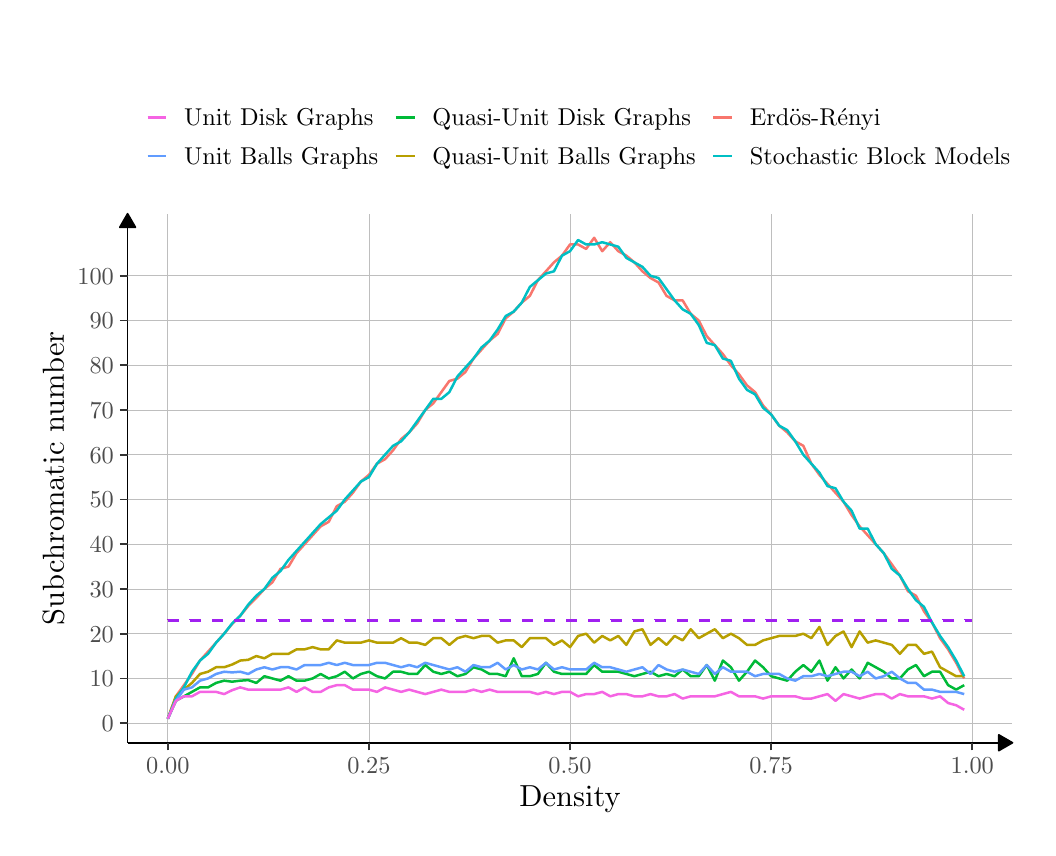
\begin{tikzpicture}[x=1pt,y=1pt]
\definecolor{fillColor}{RGB}{255,255,255}
\path[use as bounding box,fill=fillColor,fill opacity=0.00] (0,0) rectangle (361.35,289.08);
\begin{scope}
\path[clip] (  0.00,  0.00) rectangle (361.35,289.08);
\definecolor{drawColor}{RGB}{255,255,255}
\definecolor{fillColor}{RGB}{255,255,255}

\path[draw=drawColor,line width= 0.6pt,line join=round,line cap=round,fill=fillColor] (  0.00, -0.00) rectangle (361.35,289.08);
\end{scope}
\begin{scope}
\path[clip] ( 36.11, 30.69) rectangle (355.85,221.85);
\definecolor{fillColor}{RGB}{255,255,255}

\path[fill=fillColor] ( 36.11, 30.69) rectangle (355.85,221.85);
\definecolor{drawColor}{RGB}{190,190,190}

\path[draw=drawColor,line width= 0.3pt,line join=round] ( 36.11, 37.76) --
	(355.85, 37.76);

\path[draw=drawColor,line width= 0.3pt,line join=round] ( 36.11, 53.92) --
	(355.85, 53.92);

\path[draw=drawColor,line width= 0.3pt,line join=round] ( 36.11, 70.09) --
	(355.85, 70.09);

\path[draw=drawColor,line width= 0.3pt,line join=round] ( 36.11, 86.26) --
	(355.85, 86.26);

\path[draw=drawColor,line width= 0.3pt,line join=round] ( 36.11,102.42) --
	(355.85,102.42);

\path[draw=drawColor,line width= 0.3pt,line join=round] ( 36.11,118.59) --
	(355.85,118.59);

\path[draw=drawColor,line width= 0.3pt,line join=round] ( 36.11,134.76) --
	(355.85,134.76);

\path[draw=drawColor,line width= 0.3pt,line join=round] ( 36.11,150.92) --
	(355.85,150.92);

\path[draw=drawColor,line width= 0.3pt,line join=round] ( 36.11,167.09) --
	(355.85,167.09);

\path[draw=drawColor,line width= 0.3pt,line join=round] ( 36.11,183.25) --
	(355.85,183.25);

\path[draw=drawColor,line width= 0.3pt,line join=round] ( 36.11,199.42) --
	(355.85,199.42);

\path[draw=drawColor,line width= 0.3pt,line join=round] ( 50.64, 30.69) --
	( 50.64,221.85);

\path[draw=drawColor,line width= 0.3pt,line join=round] (123.31, 30.69) --
	(123.31,221.85);

\path[draw=drawColor,line width= 0.3pt,line join=round] (195.98, 30.69) --
	(195.98,221.85);

\path[draw=drawColor,line width= 0.3pt,line join=round] (268.65, 30.69) --
	(268.65,221.85);

\path[draw=drawColor,line width= 0.3pt,line join=round] (341.32, 30.69) --
	(341.32,221.85);
\definecolor{drawColor}{RGB}{248,118,109}

\path[draw=drawColor,line width= 0.9pt,line join=round] ( 50.64, 39.38) --
	( 53.55, 47.46) --
	( 56.46, 51.50) --
	( 59.36, 55.54) --
	( 62.27, 60.39) --
	( 65.18, 63.62) --
	( 68.09, 66.86) --
	( 70.99, 70.09) --
	( 73.90, 73.61) --
	( 76.81, 76.56) --
	( 79.71, 80.12) --
	( 82.62, 83.02) --
	( 85.53, 86.26) --
	( 88.43, 88.68) --
	( 91.34, 93.53) --
	( 94.25, 94.34) --
	( 97.15, 99.19) --
	(100.06,102.42) --
	(102.97,105.66) --
	(105.87,108.89) --
	(108.78,110.51) --
	(111.69,116.16) --
	(114.59,117.78) --
	(117.50,121.01) --
	(120.41,125.06) --
	(123.31,127.48) --
	(126.22,131.52) --
	(129.13,133.14) --
	(132.03,136.37) --
	(134.94,140.41) --
	(137.85,142.84) --
	(140.75,146.07) --
	(143.66,150.92) --
	(146.57,153.35) --
	(149.47,157.39) --
	(152.38,161.43) --
	(155.29,162.24) --
	(158.19,164.66) --
	(161.10,169.51) --
	(164.01,172.75) --
	(166.91,175.98) --
	(169.82,178.40) --
	(172.73,184.06) --
	(175.63,186.49) --
	(178.54,189.72) --
	(181.45,192.15) --
	(184.35,197.80) --
	(187.26,201.04) --
	(190.17,204.27) --
	(193.07,206.70) --
	(195.98,210.74) --
	(198.89,210.74) --
	(201.79,209.12) --
	(204.70,213.16) --
	(207.61,208.31) --
	(210.51,211.55) --
	(213.42,208.31) --
	(216.33,206.70) --
	(219.23,204.27) --
	(222.14,201.04) --
	(225.05,198.61) --
	(227.95,197.00) --
	(230.86,192.15) --
	(233.77,190.53) --
	(236.67,190.53) --
	(239.58,185.68) --
	(242.49,183.25) --
	(245.39,177.60) --
	(248.30,174.36) --
	(251.21,171.13) --
	(254.11,167.09) --
	(257.02,163.85) --
	(259.93,159.81) --
	(262.84,157.39) --
	(265.74,152.54) --
	(268.65,149.31) --
	(271.56,145.26) --
	(274.46,142.84) --
	(277.37,139.61) --
	(280.28,137.99) --
	(283.18,131.52) --
	(286.09,127.48) --
	(289.00,124.25) --
	(291.90,121.01) --
	(294.81,117.78) --
	(297.72,112.93) --
	(300.62,108.89) --
	(303.53,105.66) --
	(306.44,102.42) --
	(309.34, 99.19) --
	(312.25, 95.15) --
	(315.16, 91.11) --
	(318.06, 85.45) --
	(320.97, 83.83) --
	(323.88, 78.17) --
	(326.78, 74.13) --
	(329.69, 68.47) --
	(332.60, 64.43) --
	(335.50, 59.58) --
	(338.41, 53.92);
\definecolor{drawColor}{RGB}{183,159,0}

\path[draw=drawColor,line width= 0.9pt,line join=round] ( 50.64, 39.38) --
	( 53.55, 47.46) --
	( 56.46, 49.88) --
	( 59.36, 52.31) --
	( 62.27, 55.54) --
	( 65.18, 56.35) --
	( 68.09, 57.97) --
	( 70.99, 57.97) --
	( 73.90, 58.95) --
	( 76.81, 60.39) --
	( 79.71, 60.66) --
	( 82.62, 62.01) --
	( 85.53, 61.20) --
	( 88.43, 62.82) --
	( 91.34, 62.82) --
	( 94.25, 62.82) --
	( 97.15, 64.43) --
	(100.06, 64.43) --
	(102.97, 65.24) --
	(105.87, 64.43) --
	(108.78, 64.43) --
	(111.69, 67.67) --
	(114.59, 66.86) --
	(117.50, 66.86) --
	(120.41, 66.86) --
	(123.31, 67.67) --
	(126.22, 66.86) --
	(129.13, 66.86) --
	(132.03, 66.86) --
	(134.94, 68.47) --
	(137.85, 66.86) --
	(140.75, 66.86) --
	(143.66, 66.05) --
	(146.57, 68.47) --
	(149.47, 68.47) --
	(152.38, 66.05) --
	(155.29, 68.47) --
	(158.19, 69.28) --
	(161.10, 68.47) --
	(164.01, 69.28) --
	(166.91, 69.28) --
	(169.82, 66.86) --
	(172.73, 67.67) --
	(175.63, 67.67) --
	(178.54, 65.24) --
	(181.45, 68.47) --
	(184.35, 68.47) --
	(187.26, 68.47) --
	(190.17, 66.05) --
	(193.07, 67.67) --
	(195.98, 65.24) --
	(198.89, 69.28) --
	(201.79, 70.09) --
	(204.70, 66.86) --
	(207.61, 69.28) --
	(210.51, 67.67) --
	(213.42, 69.28) --
	(216.33, 66.05) --
	(219.23, 70.90) --
	(222.14, 71.71) --
	(225.05, 66.05) --
	(227.95, 68.47) --
	(230.86, 66.05) --
	(233.77, 69.28) --
	(236.67, 67.67) --
	(239.58, 71.71) --
	(242.49, 68.47) --
	(245.39, 70.09) --
	(248.30, 71.71) --
	(251.21, 68.47) --
	(254.11, 70.09) --
	(257.02, 68.47) --
	(259.93, 66.05) --
	(262.84, 66.05) --
	(265.74, 67.67) --
	(268.65, 68.47) --
	(271.56, 69.28) --
	(274.46, 69.28) --
	(277.37, 69.28) --
	(280.28, 70.09) --
	(283.18, 68.47) --
	(286.09, 72.52) --
	(289.00, 66.05) --
	(291.90, 69.28) --
	(294.81, 70.90) --
	(297.72, 65.24) --
	(300.62, 70.90) --
	(303.53, 66.86) --
	(306.44, 67.67) --
	(309.34, 66.86) --
	(312.25, 66.05) --
	(315.16, 62.82) --
	(318.06, 66.05) --
	(320.97, 66.05) --
	(323.88, 62.82) --
	(326.78, 63.62) --
	(329.69, 57.97) --
	(332.60, 56.35) --
	(335.50, 54.73) --
	(338.41, 54.73);
\definecolor{drawColor}{RGB}{0,186,56}

\path[draw=drawColor,line width= 0.9pt,line join=round] ( 50.64, 39.38) --
	( 53.55, 45.84) --
	( 56.46, 47.46) --
	( 59.36, 49.07) --
	( 62.27, 50.69) --
	( 65.18, 50.69) --
	( 68.09, 52.31) --
	( 70.99, 53.12) --
	( 73.90, 52.75) --
	( 76.81, 53.12) --
	( 79.71, 53.32) --
	( 82.62, 52.31) --
	( 85.53, 54.73) --
	( 88.43, 53.92) --
	( 91.34, 53.12) --
	( 94.25, 54.73) --
	( 97.15, 53.12) --
	(100.06, 53.12) --
	(102.97, 53.92) --
	(105.87, 55.54) --
	(108.78, 53.92) --
	(111.69, 54.73) --
	(114.59, 56.35) --
	(117.50, 53.92) --
	(120.41, 55.54) --
	(123.31, 56.35) --
	(126.22, 54.73) --
	(129.13, 53.92) --
	(132.03, 56.35) --
	(134.94, 56.35) --
	(137.85, 55.54) --
	(140.75, 55.54) --
	(143.66, 58.77) --
	(146.57, 56.35) --
	(149.47, 55.54) --
	(152.38, 56.35) --
	(155.29, 54.73) --
	(158.19, 55.54) --
	(161.10, 57.97) --
	(164.01, 57.16) --
	(166.91, 55.54) --
	(169.82, 55.54) --
	(172.73, 54.73) --
	(175.63, 61.20) --
	(178.54, 54.73) --
	(181.45, 54.73) --
	(184.35, 55.54) --
	(187.26, 59.58) --
	(190.17, 56.35) --
	(193.07, 55.54) --
	(195.98, 55.54) --
	(198.89, 55.54) --
	(201.79, 55.54) --
	(204.70, 58.77) --
	(207.61, 56.35) --
	(210.51, 56.35) --
	(213.42, 56.35) --
	(216.33, 55.54) --
	(219.23, 54.73) --
	(222.14, 55.54) --
	(225.05, 56.35) --
	(227.95, 54.73) --
	(230.86, 55.54) --
	(233.77, 54.73) --
	(236.67, 57.16) --
	(239.58, 54.73) --
	(242.49, 54.73) --
	(245.39, 58.77) --
	(248.30, 53.12) --
	(251.21, 60.39) --
	(254.11, 57.97) --
	(257.02, 53.12) --
	(259.93, 56.35) --
	(262.84, 60.39) --
	(265.74, 57.97) --
	(268.65, 54.73) --
	(271.56, 53.92) --
	(274.46, 53.12) --
	(277.37, 56.35) --
	(280.28, 58.77) --
	(283.18, 56.35) --
	(286.09, 60.39) --
	(289.00, 53.12) --
	(291.90, 57.97) --
	(294.81, 53.92) --
	(297.72, 57.16) --
	(300.62, 53.92) --
	(303.53, 59.58) --
	(306.44, 57.97) --
	(309.34, 56.35) --
	(312.25, 53.92) --
	(315.16, 53.92) --
	(318.06, 57.16) --
	(320.97, 58.77) --
	(323.88, 54.73) --
	(326.78, 56.35) --
	(329.69, 56.35) --
	(332.60, 51.50) --
	(335.50, 49.88) --
	(338.41, 51.50);
\definecolor{drawColor}{RGB}{0,191,196}

\path[draw=drawColor,line width= 0.9pt,line join=round] ( 50.64, 39.38) --
	( 53.55, 46.65) --
	( 56.46, 50.69) --
	( 59.36, 56.35) --
	( 62.27, 60.39) --
	( 65.18, 62.82) --
	( 68.09, 66.86) --
	( 70.99, 70.09) --
	( 73.90, 73.82) --
	( 76.81, 76.56) --
	( 79.71, 80.61) --
	( 82.62, 83.83) --
	( 85.53, 86.26) --
	( 88.43, 90.30) --
	( 91.34, 92.72) --
	( 94.25, 96.77) --
	( 97.15,100.00) --
	(100.06,103.23) --
	(102.97,106.46) --
	(105.87,109.70) --
	(108.78,112.12) --
	(111.69,114.55) --
	(114.59,118.59) --
	(117.50,121.82) --
	(120.41,125.06) --
	(123.31,126.67) --
	(126.22,131.52) --
	(129.13,134.76) --
	(132.03,137.99) --
	(134.94,139.61) --
	(137.85,142.84) --
	(140.75,146.88) --
	(143.66,150.92) --
	(146.57,154.96) --
	(149.47,154.96) --
	(152.38,157.39) --
	(155.29,163.05) --
	(158.19,166.28) --
	(161.10,169.51) --
	(164.01,173.55) --
	(166.91,175.98) --
	(169.82,180.02) --
	(172.73,184.87) --
	(175.63,186.49) --
	(178.54,189.72) --
	(181.45,195.38) --
	(184.35,197.80) --
	(187.26,200.23) --
	(190.17,201.04) --
	(193.07,206.70) --
	(195.98,208.31) --
	(198.89,212.35) --
	(201.79,210.74) --
	(204.70,210.74) --
	(207.61,211.55) --
	(210.51,210.74) --
	(213.42,209.93) --
	(216.33,205.89) --
	(219.23,204.27) --
	(222.14,202.65) --
	(225.05,199.42) --
	(227.95,198.61) --
	(230.86,194.57) --
	(233.77,190.53) --
	(236.67,187.30) --
	(239.58,185.68) --
	(242.49,181.64) --
	(245.39,175.17) --
	(248.30,174.36) --
	(251.21,169.51) --
	(254.11,168.70) --
	(257.02,162.24) --
	(259.93,158.20) --
	(262.84,156.58) --
	(265.74,151.73) --
	(268.65,149.31) --
	(271.56,145.26) --
	(274.46,143.65) --
	(277.37,139.61) --
	(280.28,134.76) --
	(283.18,131.52) --
	(286.09,128.29) --
	(289.00,123.44) --
	(291.90,122.63) --
	(294.81,117.78) --
	(297.72,114.55) --
	(300.62,108.08) --
	(303.53,108.08) --
	(306.44,102.42) --
	(309.34, 99.19) --
	(312.25, 93.53) --
	(315.16, 91.11) --
	(318.06, 86.26) --
	(320.97, 82.22) --
	(323.88, 79.79) --
	(326.78, 74.13) --
	(329.69, 69.28) --
	(332.60, 65.24) --
	(335.50, 60.39) --
	(338.41, 54.73);
\definecolor{drawColor}{RGB}{97,156,255}

\path[draw=drawColor,line width= 0.9pt,line join=round] ( 50.64, 39.38) --
	( 53.55, 45.84) --
	( 56.46, 49.88) --
	( 59.36, 50.69) --
	( 62.27, 53.12) --
	( 65.18, 53.92) --
	( 68.09, 55.54) --
	( 70.99, 56.35) --
	( 73.90, 56.11) --
	( 76.81, 56.35) --
	( 79.71, 55.54) --
	( 82.62, 57.16) --
	( 85.53, 57.97) --
	( 88.43, 57.16) --
	( 91.34, 57.97) --
	( 94.25, 57.97) --
	( 97.15, 57.16) --
	(100.06, 58.77) --
	(102.97, 58.77) --
	(105.87, 58.77) --
	(108.78, 59.58) --
	(111.69, 58.77) --
	(114.59, 59.58) --
	(117.50, 58.77) --
	(120.41, 58.77) --
	(123.31, 58.77) --
	(126.22, 59.58) --
	(129.13, 59.58) --
	(132.03, 58.77) --
	(134.94, 57.97) --
	(137.85, 58.77) --
	(140.75, 57.97) --
	(143.66, 59.58) --
	(146.57, 58.77) --
	(149.47, 57.97) --
	(152.38, 57.16) --
	(155.29, 57.97) --
	(158.19, 56.35) --
	(161.10, 58.77) --
	(164.01, 57.97) --
	(166.91, 57.97) --
	(169.82, 59.58) --
	(172.73, 57.16) --
	(175.63, 58.77) --
	(178.54, 57.16) --
	(181.45, 57.97) --
	(184.35, 57.16) --
	(187.26, 59.58) --
	(190.17, 57.16) --
	(193.07, 57.97) --
	(195.98, 57.16) --
	(198.89, 57.16) --
	(201.79, 57.16) --
	(204.70, 59.58) --
	(207.61, 57.97) --
	(210.51, 57.97) --
	(213.42, 57.16) --
	(216.33, 56.35) --
	(219.23, 57.16) --
	(222.14, 57.97) --
	(225.05, 55.54) --
	(227.95, 58.77) --
	(230.86, 57.16) --
	(233.77, 56.35) --
	(236.67, 57.16) --
	(239.58, 56.35) --
	(242.49, 55.54) --
	(245.39, 58.77) --
	(248.30, 55.54) --
	(251.21, 57.97) --
	(254.11, 56.35) --
	(257.02, 56.35) --
	(259.93, 56.35) --
	(262.84, 54.73) --
	(265.74, 55.54) --
	(268.65, 55.54) --
	(271.56, 55.54) --
	(274.46, 53.92) --
	(277.37, 53.12) --
	(280.28, 54.73) --
	(283.18, 54.73) --
	(286.09, 55.54) --
	(289.00, 54.73) --
	(291.90, 55.54) --
	(294.81, 56.35) --
	(297.72, 56.35) --
	(300.62, 54.73) --
	(303.53, 56.35) --
	(306.44, 53.92) --
	(309.34, 54.73) --
	(312.25, 56.35) --
	(315.16, 53.92) --
	(318.06, 52.31) --
	(320.97, 52.31) --
	(323.88, 49.88) --
	(326.78, 49.88) --
	(329.69, 49.07) --
	(332.60, 49.07) --
	(335.50, 49.07) --
	(338.41, 48.27);
\definecolor{drawColor}{RGB}{245,100,227}

\path[draw=drawColor,line width= 0.9pt,line join=round] ( 50.64, 39.38) --
	( 53.55, 45.84) --
	( 56.46, 47.46) --
	( 59.36, 47.46) --
	( 62.27, 49.07) --
	( 65.18, 49.07) --
	( 68.09, 49.07) --
	( 70.99, 48.27) --
	( 73.90, 49.69) --
	( 76.81, 50.69) --
	( 79.71, 49.88) --
	( 82.62, 49.88) --
	( 85.53, 49.88) --
	( 88.43, 49.88) --
	( 91.34, 49.88) --
	( 94.25, 50.69) --
	( 97.15, 49.07) --
	(100.06, 50.69) --
	(102.97, 49.07) --
	(105.87, 49.07) --
	(108.78, 50.69) --
	(111.69, 51.50) --
	(114.59, 51.50) --
	(117.50, 49.88) --
	(120.41, 49.88) --
	(123.31, 49.88) --
	(126.22, 49.07) --
	(129.13, 50.69) --
	(132.03, 49.88) --
	(134.94, 49.07) --
	(137.85, 49.88) --
	(140.75, 49.07) --
	(143.66, 48.27) --
	(146.57, 49.07) --
	(149.47, 49.88) --
	(152.38, 49.07) --
	(155.29, 49.07) --
	(158.19, 49.07) --
	(161.10, 49.88) --
	(164.01, 49.07) --
	(166.91, 49.88) --
	(169.82, 49.07) --
	(172.73, 49.07) --
	(175.63, 49.07) --
	(178.54, 49.07) --
	(181.45, 49.07) --
	(184.35, 48.27) --
	(187.26, 49.07) --
	(190.17, 48.27) --
	(193.07, 49.07) --
	(195.98, 49.07) --
	(198.89, 47.46) --
	(201.79, 48.27) --
	(204.70, 48.27) --
	(207.61, 49.07) --
	(210.51, 47.46) --
	(213.42, 48.27) --
	(216.33, 48.27) --
	(219.23, 47.46) --
	(222.14, 47.46) --
	(225.05, 48.27) --
	(227.95, 47.46) --
	(230.86, 47.46) --
	(233.77, 48.27) --
	(236.67, 46.65) --
	(239.58, 47.46) --
	(242.49, 47.46) --
	(245.39, 47.46) --
	(248.30, 47.46) --
	(251.21, 48.27) --
	(254.11, 49.07) --
	(257.02, 47.46) --
	(259.93, 47.46) --
	(262.84, 47.46) --
	(265.74, 46.65) --
	(268.65, 47.46) --
	(271.56, 47.46) --
	(274.46, 47.46) --
	(277.37, 47.46) --
	(280.28, 46.65) --
	(283.18, 46.65) --
	(286.09, 47.46) --
	(289.00, 48.27) --
	(291.90, 45.84) --
	(294.81, 48.27) --
	(297.72, 47.46) --
	(300.62, 46.65) --
	(303.53, 47.46) --
	(306.44, 48.27) --
	(309.34, 48.27) --
	(312.25, 46.65) --
	(315.16, 48.27) --
	(318.06, 47.46) --
	(320.97, 47.46) --
	(323.88, 47.46) --
	(326.78, 46.65) --
	(329.69, 47.46) --
	(332.60, 45.03) --
	(335.50, 44.23) --
	(338.41, 42.61);
\definecolor{drawColor}{RGB}{160,32,240}

\path[draw=drawColor,line width= 0.9pt,dash pattern=on 4pt off 4pt ,line join=round] ( 50.64, 74.94) -- (341.32, 74.94);

\path[draw=drawColor,line width= 0.9pt,dash pattern=on 4pt off 4pt ,line join=round] ( 50.64, 74.94) -- (341.32, 74.94);

\path[draw=drawColor,line width= 0.9pt,dash pattern=on 4pt off 4pt ,line join=round] ( 50.64, 74.94) -- (341.32, 74.94);

\path[draw=drawColor,line width= 0.9pt,dash pattern=on 4pt off 4pt ,line join=round] ( 50.64, 74.94) -- (341.32, 74.94);

\path[draw=drawColor,line width= 0.9pt,dash pattern=on 4pt off 4pt ,line join=round] ( 50.64, 74.94) -- (341.32, 74.94);

\path[draw=drawColor,line width= 0.9pt,dash pattern=on 4pt off 4pt ,line join=round] ( 50.64, 74.94) -- (341.32, 74.94);

\path[draw=drawColor,line width= 0.9pt,dash pattern=on 4pt off 4pt ,line join=round] ( 50.64, 74.94) -- (341.32, 74.94);

\path[draw=drawColor,line width= 0.9pt,dash pattern=on 4pt off 4pt ,line join=round] ( 50.64, 74.94) -- (341.32, 74.94);

\path[draw=drawColor,line width= 0.9pt,dash pattern=on 4pt off 4pt ,line join=round] ( 50.64, 74.94) -- (341.32, 74.94);

\path[draw=drawColor,line width= 0.9pt,dash pattern=on 4pt off 4pt ,line join=round] ( 50.64, 74.94) -- (341.32, 74.94);

\path[draw=drawColor,line width= 0.9pt,dash pattern=on 4pt off 4pt ,line join=round] ( 50.64, 74.94) -- (341.32, 74.94);

\path[draw=drawColor,line width= 0.9pt,dash pattern=on 4pt off 4pt ,line join=round] ( 50.64, 74.94) -- (341.32, 74.94);

\path[draw=drawColor,line width= 0.9pt,dash pattern=on 4pt off 4pt ,line join=round] ( 50.64, 74.94) -- (341.32, 74.94);

\path[draw=drawColor,line width= 0.9pt,dash pattern=on 4pt off 4pt ,line join=round] ( 50.64, 74.94) -- (341.32, 74.94);

\path[draw=drawColor,line width= 0.9pt,dash pattern=on 4pt off 4pt ,line join=round] ( 50.64, 74.94) -- (341.32, 74.94);

\path[draw=drawColor,line width= 0.9pt,dash pattern=on 4pt off 4pt ,line join=round] ( 50.64, 74.94) -- (341.32, 74.94);

\path[draw=drawColor,line width= 0.9pt,dash pattern=on 4pt off 4pt ,line join=round] ( 50.64, 74.94) -- (341.32, 74.94);

\path[draw=drawColor,line width= 0.9pt,dash pattern=on 4pt off 4pt ,line join=round] ( 50.64, 74.94) -- (341.32, 74.94);

\path[draw=drawColor,line width= 0.9pt,dash pattern=on 4pt off 4pt ,line join=round] ( 50.64, 74.94) -- (341.32, 74.94);

\path[draw=drawColor,line width= 0.9pt,dash pattern=on 4pt off 4pt ,line join=round] ( 50.64, 74.94) -- (341.32, 74.94);

\path[draw=drawColor,line width= 0.9pt,dash pattern=on 4pt off 4pt ,line join=round] ( 50.64, 74.94) -- (341.32, 74.94);

\path[draw=drawColor,line width= 0.9pt,dash pattern=on 4pt off 4pt ,line join=round] ( 50.64, 74.94) -- (341.32, 74.94);

\path[draw=drawColor,line width= 0.9pt,dash pattern=on 4pt off 4pt ,line join=round] ( 50.64, 74.94) -- (341.32, 74.94);

\path[draw=drawColor,line width= 0.9pt,dash pattern=on 4pt off 4pt ,line join=round] ( 50.64, 74.94) -- (341.32, 74.94);

\path[draw=drawColor,line width= 0.9pt,dash pattern=on 4pt off 4pt ,line join=round] ( 50.64, 74.94) -- (341.32, 74.94);

\path[draw=drawColor,line width= 0.9pt,dash pattern=on 4pt off 4pt ,line join=round] ( 50.64, 74.94) -- (341.32, 74.94);

\path[draw=drawColor,line width= 0.9pt,dash pattern=on 4pt off 4pt ,line join=round] ( 50.64, 74.94) -- (341.32, 74.94);

\path[draw=drawColor,line width= 0.9pt,dash pattern=on 4pt off 4pt ,line join=round] ( 50.64, 74.94) -- (341.32, 74.94);

\path[draw=drawColor,line width= 0.9pt,dash pattern=on 4pt off 4pt ,line join=round] ( 50.64, 74.94) -- (341.32, 74.94);

\path[draw=drawColor,line width= 0.9pt,dash pattern=on 4pt off 4pt ,line join=round] ( 50.64, 74.94) -- (341.32, 74.94);

\path[draw=drawColor,line width= 0.9pt,dash pattern=on 4pt off 4pt ,line join=round] ( 50.64, 74.94) -- (341.32, 74.94);

\path[draw=drawColor,line width= 0.9pt,dash pattern=on 4pt off 4pt ,line join=round] ( 50.64, 74.94) -- (341.32, 74.94);

\path[draw=drawColor,line width= 0.9pt,dash pattern=on 4pt off 4pt ,line join=round] ( 50.64, 74.94) -- (341.32, 74.94);

\path[draw=drawColor,line width= 0.9pt,dash pattern=on 4pt off 4pt ,line join=round] ( 50.64, 74.94) -- (341.32, 74.94);

\path[draw=drawColor,line width= 0.9pt,dash pattern=on 4pt off 4pt ,line join=round] ( 50.64, 74.94) -- (341.32, 74.94);

\path[draw=drawColor,line width= 0.9pt,dash pattern=on 4pt off 4pt ,line join=round] ( 50.64, 74.94) -- (341.32, 74.94);

\path[draw=drawColor,line width= 0.9pt,dash pattern=on 4pt off 4pt ,line join=round] ( 50.64, 74.94) -- (341.32, 74.94);

\path[draw=drawColor,line width= 0.9pt,dash pattern=on 4pt off 4pt ,line join=round] ( 50.64, 74.94) -- (341.32, 74.94);

\path[draw=drawColor,line width= 0.9pt,dash pattern=on 4pt off 4pt ,line join=round] ( 50.64, 74.94) -- (341.32, 74.94);

\path[draw=drawColor,line width= 0.9pt,dash pattern=on 4pt off 4pt ,line join=round] ( 50.64, 74.94) -- (341.32, 74.94);

\path[draw=drawColor,line width= 0.9pt,dash pattern=on 4pt off 4pt ,line join=round] ( 50.64, 74.94) -- (341.32, 74.94);

\path[draw=drawColor,line width= 0.9pt,dash pattern=on 4pt off 4pt ,line join=round] ( 50.64, 74.94) -- (341.32, 74.94);

\path[draw=drawColor,line width= 0.9pt,dash pattern=on 4pt off 4pt ,line join=round] ( 50.64, 74.94) -- (341.32, 74.94);

\path[draw=drawColor,line width= 0.9pt,dash pattern=on 4pt off 4pt ,line join=round] ( 50.64, 74.94) -- (341.32, 74.94);

\path[draw=drawColor,line width= 0.9pt,dash pattern=on 4pt off 4pt ,line join=round] ( 50.64, 74.94) -- (341.32, 74.94);

\path[draw=drawColor,line width= 0.9pt,dash pattern=on 4pt off 4pt ,line join=round] ( 50.64, 74.94) -- (341.32, 74.94);

\path[draw=drawColor,line width= 0.9pt,dash pattern=on 4pt off 4pt ,line join=round] ( 50.64, 74.94) -- (341.32, 74.94);

\path[draw=drawColor,line width= 0.9pt,dash pattern=on 4pt off 4pt ,line join=round] ( 50.64, 74.94) -- (341.32, 74.94);

\path[draw=drawColor,line width= 0.9pt,dash pattern=on 4pt off 4pt ,line join=round] ( 50.64, 74.94) -- (341.32, 74.94);

\path[draw=drawColor,line width= 0.9pt,dash pattern=on 4pt off 4pt ,line join=round] ( 50.64, 74.94) -- (341.32, 74.94);

\path[draw=drawColor,line width= 0.9pt,dash pattern=on 4pt off 4pt ,line join=round] ( 50.64, 74.94) -- (341.32, 74.94);

\path[draw=drawColor,line width= 0.9pt,dash pattern=on 4pt off 4pt ,line join=round] ( 50.64, 74.94) -- (341.32, 74.94);

\path[draw=drawColor,line width= 0.9pt,dash pattern=on 4pt off 4pt ,line join=round] ( 50.64, 74.94) -- (341.32, 74.94);

\path[draw=drawColor,line width= 0.9pt,dash pattern=on 4pt off 4pt ,line join=round] ( 50.64, 74.94) -- (341.32, 74.94);

\path[draw=drawColor,line width= 0.9pt,dash pattern=on 4pt off 4pt ,line join=round] ( 50.64, 74.94) -- (341.32, 74.94);

\path[draw=drawColor,line width= 0.9pt,dash pattern=on 4pt off 4pt ,line join=round] ( 50.64, 74.94) -- (341.32, 74.94);

\path[draw=drawColor,line width= 0.9pt,dash pattern=on 4pt off 4pt ,line join=round] ( 50.64, 74.94) -- (341.32, 74.94);

\path[draw=drawColor,line width= 0.9pt,dash pattern=on 4pt off 4pt ,line join=round] ( 50.64, 74.94) -- (341.32, 74.94);

\path[draw=drawColor,line width= 0.9pt,dash pattern=on 4pt off 4pt ,line join=round] ( 50.64, 74.94) -- (341.32, 74.94);

\path[draw=drawColor,line width= 0.9pt,dash pattern=on 4pt off 4pt ,line join=round] ( 50.64, 74.94) -- (341.32, 74.94);

\path[draw=drawColor,line width= 0.9pt,dash pattern=on 4pt off 4pt ,line join=round] ( 50.64, 74.94) -- (341.32, 74.94);

\path[draw=drawColor,line width= 0.9pt,dash pattern=on 4pt off 4pt ,line join=round] ( 50.64, 74.94) -- (341.32, 74.94);

\path[draw=drawColor,line width= 0.9pt,dash pattern=on 4pt off 4pt ,line join=round] ( 50.64, 74.94) -- (341.32, 74.94);

\path[draw=drawColor,line width= 0.9pt,dash pattern=on 4pt off 4pt ,line join=round] ( 50.64, 74.94) -- (341.32, 74.94);

\path[draw=drawColor,line width= 0.9pt,dash pattern=on 4pt off 4pt ,line join=round] ( 50.64, 74.94) -- (341.32, 74.94);

\path[draw=drawColor,line width= 0.9pt,dash pattern=on 4pt off 4pt ,line join=round] ( 50.64, 74.94) -- (341.32, 74.94);

\path[draw=drawColor,line width= 0.9pt,dash pattern=on 4pt off 4pt ,line join=round] ( 50.64, 74.94) -- (341.32, 74.94);

\path[draw=drawColor,line width= 0.9pt,dash pattern=on 4pt off 4pt ,line join=round] ( 50.64, 74.94) -- (341.32, 74.94);

\path[draw=drawColor,line width= 0.9pt,dash pattern=on 4pt off 4pt ,line join=round] ( 50.64, 74.94) -- (341.32, 74.94);

\path[draw=drawColor,line width= 0.9pt,dash pattern=on 4pt off 4pt ,line join=round] ( 50.64, 74.94) -- (341.32, 74.94);

\path[draw=drawColor,line width= 0.9pt,dash pattern=on 4pt off 4pt ,line join=round] ( 50.64, 74.94) -- (341.32, 74.94);

\path[draw=drawColor,line width= 0.9pt,dash pattern=on 4pt off 4pt ,line join=round] ( 50.64, 74.94) -- (341.32, 74.94);

\path[draw=drawColor,line width= 0.9pt,dash pattern=on 4pt off 4pt ,line join=round] ( 50.64, 74.94) -- (341.32, 74.94);

\path[draw=drawColor,line width= 0.9pt,dash pattern=on 4pt off 4pt ,line join=round] ( 50.64, 74.94) -- (341.32, 74.94);

\path[draw=drawColor,line width= 0.9pt,dash pattern=on 4pt off 4pt ,line join=round] ( 50.64, 74.94) -- (341.32, 74.94);

\path[draw=drawColor,line width= 0.9pt,dash pattern=on 4pt off 4pt ,line join=round] ( 50.64, 74.94) -- (341.32, 74.94);

\path[draw=drawColor,line width= 0.9pt,dash pattern=on 4pt off 4pt ,line join=round] ( 50.64, 74.94) -- (341.32, 74.94);

\path[draw=drawColor,line width= 0.9pt,dash pattern=on 4pt off 4pt ,line join=round] ( 50.64, 74.94) -- (341.32, 74.94);

\path[draw=drawColor,line width= 0.9pt,dash pattern=on 4pt off 4pt ,line join=round] ( 50.64, 74.94) -- (341.32, 74.94);

\path[draw=drawColor,line width= 0.9pt,dash pattern=on 4pt off 4pt ,line join=round] ( 50.64, 74.94) -- (341.32, 74.94);

\path[draw=drawColor,line width= 0.9pt,dash pattern=on 4pt off 4pt ,line join=round] ( 50.64, 74.94) -- (341.32, 74.94);

\path[draw=drawColor,line width= 0.9pt,dash pattern=on 4pt off 4pt ,line join=round] ( 50.64, 74.94) -- (341.32, 74.94);

\path[draw=drawColor,line width= 0.9pt,dash pattern=on 4pt off 4pt ,line join=round] ( 50.64, 74.94) -- (341.32, 74.94);

\path[draw=drawColor,line width= 0.9pt,dash pattern=on 4pt off 4pt ,line join=round] ( 50.64, 74.94) -- (341.32, 74.94);

\path[draw=drawColor,line width= 0.9pt,dash pattern=on 4pt off 4pt ,line join=round] ( 50.64, 74.94) -- (341.32, 74.94);

\path[draw=drawColor,line width= 0.9pt,dash pattern=on 4pt off 4pt ,line join=round] ( 50.64, 74.94) -- (341.32, 74.94);

\path[draw=drawColor,line width= 0.9pt,dash pattern=on 4pt off 4pt ,line join=round] ( 50.64, 74.94) -- (341.32, 74.94);

\path[draw=drawColor,line width= 0.9pt,dash pattern=on 4pt off 4pt ,line join=round] ( 50.64, 74.94) -- (341.32, 74.94);

\path[draw=drawColor,line width= 0.9pt,dash pattern=on 4pt off 4pt ,line join=round] ( 50.64, 74.94) -- (341.32, 74.94);

\path[draw=drawColor,line width= 0.9pt,dash pattern=on 4pt off 4pt ,line join=round] ( 50.64, 74.94) -- (341.32, 74.94);

\path[draw=drawColor,line width= 0.9pt,dash pattern=on 4pt off 4pt ,line join=round] ( 50.64, 74.94) -- (341.32, 74.94);

\path[draw=drawColor,line width= 0.9pt,dash pattern=on 4pt off 4pt ,line join=round] ( 50.64, 74.94) -- (341.32, 74.94);

\path[draw=drawColor,line width= 0.9pt,dash pattern=on 4pt off 4pt ,line join=round] ( 50.64, 74.94) -- (341.32, 74.94);

\path[draw=drawColor,line width= 0.9pt,dash pattern=on 4pt off 4pt ,line join=round] ( 50.64, 74.94) -- (341.32, 74.94);

\path[draw=drawColor,line width= 0.9pt,dash pattern=on 4pt off 4pt ,line join=round] ( 50.64, 74.94) -- (341.32, 74.94);

\path[draw=drawColor,line width= 0.9pt,dash pattern=on 4pt off 4pt ,line join=round] ( 50.64, 74.94) -- (341.32, 74.94);

\path[draw=drawColor,line width= 0.9pt,dash pattern=on 4pt off 4pt ,line join=round] ( 50.64, 74.94) -- (341.32, 74.94);

\path[draw=drawColor,line width= 0.9pt,dash pattern=on 4pt off 4pt ,line join=round] ( 50.64, 74.94) -- (341.32, 74.94);

\path[draw=drawColor,line width= 0.9pt,dash pattern=on 4pt off 4pt ,line join=round] ( 50.64, 74.94) -- (341.32, 74.94);

\path[draw=drawColor,line width= 0.9pt,dash pattern=on 4pt off 4pt ,line join=round] ( 50.64, 74.94) -- (341.32, 74.94);

\path[draw=drawColor,line width= 0.9pt,dash pattern=on 4pt off 4pt ,line join=round] ( 50.64, 74.94) -- (341.32, 74.94);

\path[draw=drawColor,line width= 0.9pt,dash pattern=on 4pt off 4pt ,line join=round] ( 50.64, 74.94) -- (341.32, 74.94);

\path[draw=drawColor,line width= 0.9pt,dash pattern=on 4pt off 4pt ,line join=round] ( 50.64, 74.94) -- (341.32, 74.94);

\path[draw=drawColor,line width= 0.9pt,dash pattern=on 4pt off 4pt ,line join=round] ( 50.64, 74.94) -- (341.32, 74.94);

\path[draw=drawColor,line width= 0.9pt,dash pattern=on 4pt off 4pt ,line join=round] ( 50.64, 74.94) -- (341.32, 74.94);

\path[draw=drawColor,line width= 0.9pt,dash pattern=on 4pt off 4pt ,line join=round] ( 50.64, 74.94) -- (341.32, 74.94);

\path[draw=drawColor,line width= 0.9pt,dash pattern=on 4pt off 4pt ,line join=round] ( 50.64, 74.94) -- (341.32, 74.94);

\path[draw=drawColor,line width= 0.9pt,dash pattern=on 4pt off 4pt ,line join=round] ( 50.64, 74.94) -- (341.32, 74.94);

\path[draw=drawColor,line width= 0.9pt,dash pattern=on 4pt off 4pt ,line join=round] ( 50.64, 74.94) -- (341.32, 74.94);

\path[draw=drawColor,line width= 0.9pt,dash pattern=on 4pt off 4pt ,line join=round] ( 50.64, 74.94) -- (341.32, 74.94);

\path[draw=drawColor,line width= 0.9pt,dash pattern=on 4pt off 4pt ,line join=round] ( 50.64, 74.94) -- (341.32, 74.94);

\path[draw=drawColor,line width= 0.9pt,dash pattern=on 4pt off 4pt ,line join=round] ( 50.64, 74.94) -- (341.32, 74.94);

\path[draw=drawColor,line width= 0.9pt,dash pattern=on 4pt off 4pt ,line join=round] ( 50.64, 74.94) -- (341.32, 74.94);

\path[draw=drawColor,line width= 0.9pt,dash pattern=on 4pt off 4pt ,line join=round] ( 50.64, 74.94) -- (341.32, 74.94);

\path[draw=drawColor,line width= 0.9pt,dash pattern=on 4pt off 4pt ,line join=round] ( 50.64, 74.94) -- (341.32, 74.94);

\path[draw=drawColor,line width= 0.9pt,dash pattern=on 4pt off 4pt ,line join=round] ( 50.64, 74.94) -- (341.32, 74.94);

\path[draw=drawColor,line width= 0.9pt,dash pattern=on 4pt off 4pt ,line join=round] ( 50.64, 74.94) -- (341.32, 74.94);

\path[draw=drawColor,line width= 0.9pt,dash pattern=on 4pt off 4pt ,line join=round] ( 50.64, 74.94) -- (341.32, 74.94);

\path[draw=drawColor,line width= 0.9pt,dash pattern=on 4pt off 4pt ,line join=round] ( 50.64, 74.94) -- (341.32, 74.94);

\path[draw=drawColor,line width= 0.9pt,dash pattern=on 4pt off 4pt ,line join=round] ( 50.64, 74.94) -- (341.32, 74.94);

\path[draw=drawColor,line width= 0.9pt,dash pattern=on 4pt off 4pt ,line join=round] ( 50.64, 74.94) -- (341.32, 74.94);

\path[draw=drawColor,line width= 0.9pt,dash pattern=on 4pt off 4pt ,line join=round] ( 50.64, 74.94) -- (341.32, 74.94);

\path[draw=drawColor,line width= 0.9pt,dash pattern=on 4pt off 4pt ,line join=round] ( 50.64, 74.94) -- (341.32, 74.94);

\path[draw=drawColor,line width= 0.9pt,dash pattern=on 4pt off 4pt ,line join=round] ( 50.64, 74.94) -- (341.32, 74.94);

\path[draw=drawColor,line width= 0.9pt,dash pattern=on 4pt off 4pt ,line join=round] ( 50.64, 74.94) -- (341.32, 74.94);

\path[draw=drawColor,line width= 0.9pt,dash pattern=on 4pt off 4pt ,line join=round] ( 50.64, 74.94) -- (341.32, 74.94);

\path[draw=drawColor,line width= 0.9pt,dash pattern=on 4pt off 4pt ,line join=round] ( 50.64, 74.94) -- (341.32, 74.94);

\path[draw=drawColor,line width= 0.9pt,dash pattern=on 4pt off 4pt ,line join=round] ( 50.64, 74.94) -- (341.32, 74.94);

\path[draw=drawColor,line width= 0.9pt,dash pattern=on 4pt off 4pt ,line join=round] ( 50.64, 74.94) -- (341.32, 74.94);

\path[draw=drawColor,line width= 0.9pt,dash pattern=on 4pt off 4pt ,line join=round] ( 50.64, 74.94) -- (341.32, 74.94);

\path[draw=drawColor,line width= 0.9pt,dash pattern=on 4pt off 4pt ,line join=round] ( 50.64, 74.94) -- (341.32, 74.94);

\path[draw=drawColor,line width= 0.9pt,dash pattern=on 4pt off 4pt ,line join=round] ( 50.64, 74.94) -- (341.32, 74.94);

\path[draw=drawColor,line width= 0.9pt,dash pattern=on 4pt off 4pt ,line join=round] ( 50.64, 74.94) -- (341.32, 74.94);

\path[draw=drawColor,line width= 0.9pt,dash pattern=on 4pt off 4pt ,line join=round] ( 50.64, 74.94) -- (341.32, 74.94);

\path[draw=drawColor,line width= 0.9pt,dash pattern=on 4pt off 4pt ,line join=round] ( 50.64, 74.94) -- (341.32, 74.94);

\path[draw=drawColor,line width= 0.9pt,dash pattern=on 4pt off 4pt ,line join=round] ( 50.64, 74.94) -- (341.32, 74.94);

\path[draw=drawColor,line width= 0.9pt,dash pattern=on 4pt off 4pt ,line join=round] ( 50.64, 74.94) -- (341.32, 74.94);

\path[draw=drawColor,line width= 0.9pt,dash pattern=on 4pt off 4pt ,line join=round] ( 50.64, 74.94) -- (341.32, 74.94);

\path[draw=drawColor,line width= 0.9pt,dash pattern=on 4pt off 4pt ,line join=round] ( 50.64, 74.94) -- (341.32, 74.94);

\path[draw=drawColor,line width= 0.9pt,dash pattern=on 4pt off 4pt ,line join=round] ( 50.64, 74.94) -- (341.32, 74.94);

\path[draw=drawColor,line width= 0.9pt,dash pattern=on 4pt off 4pt ,line join=round] ( 50.64, 74.94) -- (341.32, 74.94);

\path[draw=drawColor,line width= 0.9pt,dash pattern=on 4pt off 4pt ,line join=round] ( 50.64, 74.94) -- (341.32, 74.94);

\path[draw=drawColor,line width= 0.9pt,dash pattern=on 4pt off 4pt ,line join=round] ( 50.64, 74.94) -- (341.32, 74.94);

\path[draw=drawColor,line width= 0.9pt,dash pattern=on 4pt off 4pt ,line join=round] ( 50.64, 74.94) -- (341.32, 74.94);

\path[draw=drawColor,line width= 0.9pt,dash pattern=on 4pt off 4pt ,line join=round] ( 50.64, 74.94) -- (341.32, 74.94);

\path[draw=drawColor,line width= 0.9pt,dash pattern=on 4pt off 4pt ,line join=round] ( 50.64, 74.94) -- (341.32, 74.94);

\path[draw=drawColor,line width= 0.9pt,dash pattern=on 4pt off 4pt ,line join=round] ( 50.64, 74.94) -- (341.32, 74.94);

\path[draw=drawColor,line width= 0.9pt,dash pattern=on 4pt off 4pt ,line join=round] ( 50.64, 74.94) -- (341.32, 74.94);

\path[draw=drawColor,line width= 0.9pt,dash pattern=on 4pt off 4pt ,line join=round] ( 50.64, 74.94) -- (341.32, 74.94);

\path[draw=drawColor,line width= 0.9pt,dash pattern=on 4pt off 4pt ,line join=round] ( 50.64, 74.94) -- (341.32, 74.94);

\path[draw=drawColor,line width= 0.9pt,dash pattern=on 4pt off 4pt ,line join=round] ( 50.64, 74.94) -- (341.32, 74.94);

\path[draw=drawColor,line width= 0.9pt,dash pattern=on 4pt off 4pt ,line join=round] ( 50.64, 74.94) -- (341.32, 74.94);

\path[draw=drawColor,line width= 0.9pt,dash pattern=on 4pt off 4pt ,line join=round] ( 50.64, 74.94) -- (341.32, 74.94);

\path[draw=drawColor,line width= 0.9pt,dash pattern=on 4pt off 4pt ,line join=round] ( 50.64, 74.94) -- (341.32, 74.94);

\path[draw=drawColor,line width= 0.9pt,dash pattern=on 4pt off 4pt ,line join=round] ( 50.64, 74.94) -- (341.32, 74.94);

\path[draw=drawColor,line width= 0.9pt,dash pattern=on 4pt off 4pt ,line join=round] ( 50.64, 74.94) -- (341.32, 74.94);

\path[draw=drawColor,line width= 0.9pt,dash pattern=on 4pt off 4pt ,line join=round] ( 50.64, 74.94) -- (341.32, 74.94);

\path[draw=drawColor,line width= 0.9pt,dash pattern=on 4pt off 4pt ,line join=round] ( 50.64, 74.94) -- (341.32, 74.94);

\path[draw=drawColor,line width= 0.9pt,dash pattern=on 4pt off 4pt ,line join=round] ( 50.64, 74.94) -- (341.32, 74.94);

\path[draw=drawColor,line width= 0.9pt,dash pattern=on 4pt off 4pt ,line join=round] ( 50.64, 74.94) -- (341.32, 74.94);

\path[draw=drawColor,line width= 0.9pt,dash pattern=on 4pt off 4pt ,line join=round] ( 50.64, 74.94) -- (341.32, 74.94);

\path[draw=drawColor,line width= 0.9pt,dash pattern=on 4pt off 4pt ,line join=round] ( 50.64, 74.94) -- (341.32, 74.94);

\path[draw=drawColor,line width= 0.9pt,dash pattern=on 4pt off 4pt ,line join=round] ( 50.64, 74.94) -- (341.32, 74.94);

\path[draw=drawColor,line width= 0.9pt,dash pattern=on 4pt off 4pt ,line join=round] ( 50.64, 74.94) -- (341.32, 74.94);

\path[draw=drawColor,line width= 0.9pt,dash pattern=on 4pt off 4pt ,line join=round] ( 50.64, 74.94) -- (341.32, 74.94);

\path[draw=drawColor,line width= 0.9pt,dash pattern=on 4pt off 4pt ,line join=round] ( 50.64, 74.94) -- (341.32, 74.94);

\path[draw=drawColor,line width= 0.9pt,dash pattern=on 4pt off 4pt ,line join=round] ( 50.64, 74.94) -- (341.32, 74.94);

\path[draw=drawColor,line width= 0.9pt,dash pattern=on 4pt off 4pt ,line join=round] ( 50.64, 74.94) -- (341.32, 74.94);

\path[draw=drawColor,line width= 0.9pt,dash pattern=on 4pt off 4pt ,line join=round] ( 50.64, 74.94) -- (341.32, 74.94);

\path[draw=drawColor,line width= 0.9pt,dash pattern=on 4pt off 4pt ,line join=round] ( 50.64, 74.94) -- (341.32, 74.94);

\path[draw=drawColor,line width= 0.9pt,dash pattern=on 4pt off 4pt ,line join=round] ( 50.64, 74.94) -- (341.32, 74.94);

\path[draw=drawColor,line width= 0.9pt,dash pattern=on 4pt off 4pt ,line join=round] ( 50.64, 74.94) -- (341.32, 74.94);

\path[draw=drawColor,line width= 0.9pt,dash pattern=on 4pt off 4pt ,line join=round] ( 50.64, 74.94) -- (341.32, 74.94);

\path[draw=drawColor,line width= 0.9pt,dash pattern=on 4pt off 4pt ,line join=round] ( 50.64, 74.94) -- (341.32, 74.94);

\path[draw=drawColor,line width= 0.9pt,dash pattern=on 4pt off 4pt ,line join=round] ( 50.64, 74.94) -- (341.32, 74.94);

\path[draw=drawColor,line width= 0.9pt,dash pattern=on 4pt off 4pt ,line join=round] ( 50.64, 74.94) -- (341.32, 74.94);

\path[draw=drawColor,line width= 0.9pt,dash pattern=on 4pt off 4pt ,line join=round] ( 50.64, 74.94) -- (341.32, 74.94);

\path[draw=drawColor,line width= 0.9pt,dash pattern=on 4pt off 4pt ,line join=round] ( 50.64, 74.94) -- (341.32, 74.94);

\path[draw=drawColor,line width= 0.9pt,dash pattern=on 4pt off 4pt ,line join=round] ( 50.64, 74.94) -- (341.32, 74.94);

\path[draw=drawColor,line width= 0.9pt,dash pattern=on 4pt off 4pt ,line join=round] ( 50.64, 74.94) -- (341.32, 74.94);

\path[draw=drawColor,line width= 0.9pt,dash pattern=on 4pt off 4pt ,line join=round] ( 50.64, 74.94) -- (341.32, 74.94);

\path[draw=drawColor,line width= 0.9pt,dash pattern=on 4pt off 4pt ,line join=round] ( 50.64, 74.94) -- (341.32, 74.94);

\path[draw=drawColor,line width= 0.9pt,dash pattern=on 4pt off 4pt ,line join=round] ( 50.64, 74.94) -- (341.32, 74.94);

\path[draw=drawColor,line width= 0.9pt,dash pattern=on 4pt off 4pt ,line join=round] ( 50.64, 74.94) -- (341.32, 74.94);

\path[draw=drawColor,line width= 0.9pt,dash pattern=on 4pt off 4pt ,line join=round] ( 50.64, 74.94) -- (341.32, 74.94);

\path[draw=drawColor,line width= 0.9pt,dash pattern=on 4pt off 4pt ,line join=round] ( 50.64, 74.94) -- (341.32, 74.94);

\path[draw=drawColor,line width= 0.9pt,dash pattern=on 4pt off 4pt ,line join=round] ( 50.64, 74.94) -- (341.32, 74.94);

\path[draw=drawColor,line width= 0.9pt,dash pattern=on 4pt off 4pt ,line join=round] ( 50.64, 74.94) -- (341.32, 74.94);

\path[draw=drawColor,line width= 0.9pt,dash pattern=on 4pt off 4pt ,line join=round] ( 50.64, 74.94) -- (341.32, 74.94);

\path[draw=drawColor,line width= 0.9pt,dash pattern=on 4pt off 4pt ,line join=round] ( 50.64, 74.94) -- (341.32, 74.94);

\path[draw=drawColor,line width= 0.9pt,dash pattern=on 4pt off 4pt ,line join=round] ( 50.64, 74.94) -- (341.32, 74.94);

\path[draw=drawColor,line width= 0.9pt,dash pattern=on 4pt off 4pt ,line join=round] ( 50.64, 74.94) -- (341.32, 74.94);

\path[draw=drawColor,line width= 0.9pt,dash pattern=on 4pt off 4pt ,line join=round] ( 50.64, 74.94) -- (341.32, 74.94);

\path[draw=drawColor,line width= 0.9pt,dash pattern=on 4pt off 4pt ,line join=round] ( 50.64, 74.94) -- (341.32, 74.94);

\path[draw=drawColor,line width= 0.9pt,dash pattern=on 4pt off 4pt ,line join=round] ( 50.64, 74.94) -- (341.32, 74.94);

\path[draw=drawColor,line width= 0.9pt,dash pattern=on 4pt off 4pt ,line join=round] ( 50.64, 74.94) -- (341.32, 74.94);

\path[draw=drawColor,line width= 0.9pt,dash pattern=on 4pt off 4pt ,line join=round] ( 50.64, 74.94) -- (341.32, 74.94);

\path[draw=drawColor,line width= 0.9pt,dash pattern=on 4pt off 4pt ,line join=round] ( 50.64, 74.94) -- (341.32, 74.94);

\path[draw=drawColor,line width= 0.9pt,dash pattern=on 4pt off 4pt ,line join=round] ( 50.64, 74.94) -- (341.32, 74.94);

\path[draw=drawColor,line width= 0.9pt,dash pattern=on 4pt off 4pt ,line join=round] ( 50.64, 74.94) -- (341.32, 74.94);

\path[draw=drawColor,line width= 0.9pt,dash pattern=on 4pt off 4pt ,line join=round] ( 50.64, 74.94) -- (341.32, 74.94);

\path[draw=drawColor,line width= 0.9pt,dash pattern=on 4pt off 4pt ,line join=round] ( 50.64, 74.94) -- (341.32, 74.94);

\path[draw=drawColor,line width= 0.9pt,dash pattern=on 4pt off 4pt ,line join=round] ( 50.64, 74.94) -- (341.32, 74.94);

\path[draw=drawColor,line width= 0.9pt,dash pattern=on 4pt off 4pt ,line join=round] ( 50.64, 74.94) -- (341.32, 74.94);

\path[draw=drawColor,line width= 0.9pt,dash pattern=on 4pt off 4pt ,line join=round] ( 50.64, 74.94) -- (341.32, 74.94);

\path[draw=drawColor,line width= 0.9pt,dash pattern=on 4pt off 4pt ,line join=round] ( 50.64, 74.94) -- (341.32, 74.94);

\path[draw=drawColor,line width= 0.9pt,dash pattern=on 4pt off 4pt ,line join=round] ( 50.64, 74.94) -- (341.32, 74.94);

\path[draw=drawColor,line width= 0.9pt,dash pattern=on 4pt off 4pt ,line join=round] ( 50.64, 74.94) -- (341.32, 74.94);

\path[draw=drawColor,line width= 0.9pt,dash pattern=on 4pt off 4pt ,line join=round] ( 50.64, 74.94) -- (341.32, 74.94);

\path[draw=drawColor,line width= 0.9pt,dash pattern=on 4pt off 4pt ,line join=round] ( 50.64, 74.94) -- (341.32, 74.94);

\path[draw=drawColor,line width= 0.9pt,dash pattern=on 4pt off 4pt ,line join=round] ( 50.64, 74.94) -- (341.32, 74.94);

\path[draw=drawColor,line width= 0.9pt,dash pattern=on 4pt off 4pt ,line join=round] ( 50.64, 74.94) -- (341.32, 74.94);

\path[draw=drawColor,line width= 0.9pt,dash pattern=on 4pt off 4pt ,line join=round] ( 50.64, 74.94) -- (341.32, 74.94);

\path[draw=drawColor,line width= 0.9pt,dash pattern=on 4pt off 4pt ,line join=round] ( 50.64, 74.94) -- (341.32, 74.94);

\path[draw=drawColor,line width= 0.9pt,dash pattern=on 4pt off 4pt ,line join=round] ( 50.64, 74.94) -- (341.32, 74.94);

\path[draw=drawColor,line width= 0.9pt,dash pattern=on 4pt off 4pt ,line join=round] ( 50.64, 74.94) -- (341.32, 74.94);

\path[draw=drawColor,line width= 0.9pt,dash pattern=on 4pt off 4pt ,line join=round] ( 50.64, 74.94) -- (341.32, 74.94);

\path[draw=drawColor,line width= 0.9pt,dash pattern=on 4pt off 4pt ,line join=round] ( 50.64, 74.94) -- (341.32, 74.94);

\path[draw=drawColor,line width= 0.9pt,dash pattern=on 4pt off 4pt ,line join=round] ( 50.64, 74.94) -- (341.32, 74.94);

\path[draw=drawColor,line width= 0.9pt,dash pattern=on 4pt off 4pt ,line join=round] ( 50.64, 74.94) -- (341.32, 74.94);

\path[draw=drawColor,line width= 0.9pt,dash pattern=on 4pt off 4pt ,line join=round] ( 50.64, 74.94) -- (341.32, 74.94);

\path[draw=drawColor,line width= 0.9pt,dash pattern=on 4pt off 4pt ,line join=round] ( 50.64, 74.94) -- (341.32, 74.94);

\path[draw=drawColor,line width= 0.9pt,dash pattern=on 4pt off 4pt ,line join=round] ( 50.64, 74.94) -- (341.32, 74.94);

\path[draw=drawColor,line width= 0.9pt,dash pattern=on 4pt off 4pt ,line join=round] ( 50.64, 74.94) -- (341.32, 74.94);

\path[draw=drawColor,line width= 0.9pt,dash pattern=on 4pt off 4pt ,line join=round] ( 50.64, 74.94) -- (341.32, 74.94);

\path[draw=drawColor,line width= 0.9pt,dash pattern=on 4pt off 4pt ,line join=round] ( 50.64, 74.94) -- (341.32, 74.94);

\path[draw=drawColor,line width= 0.9pt,dash pattern=on 4pt off 4pt ,line join=round] ( 50.64, 74.94) -- (341.32, 74.94);

\path[draw=drawColor,line width= 0.9pt,dash pattern=on 4pt off 4pt ,line join=round] ( 50.64, 74.94) -- (341.32, 74.94);

\path[draw=drawColor,line width= 0.9pt,dash pattern=on 4pt off 4pt ,line join=round] ( 50.64, 74.94) -- (341.32, 74.94);

\path[draw=drawColor,line width= 0.9pt,dash pattern=on 4pt off 4pt ,line join=round] ( 50.64, 74.94) -- (341.32, 74.94);

\path[draw=drawColor,line width= 0.9pt,dash pattern=on 4pt off 4pt ,line join=round] ( 50.64, 74.94) -- (341.32, 74.94);

\path[draw=drawColor,line width= 0.9pt,dash pattern=on 4pt off 4pt ,line join=round] ( 50.64, 74.94) -- (341.32, 74.94);

\path[draw=drawColor,line width= 0.9pt,dash pattern=on 4pt off 4pt ,line join=round] ( 50.64, 74.94) -- (341.32, 74.94);

\path[draw=drawColor,line width= 0.9pt,dash pattern=on 4pt off 4pt ,line join=round] ( 50.64, 74.94) -- (341.32, 74.94);

\path[draw=drawColor,line width= 0.9pt,dash pattern=on 4pt off 4pt ,line join=round] ( 50.64, 74.94) -- (341.32, 74.94);

\path[draw=drawColor,line width= 0.9pt,dash pattern=on 4pt off 4pt ,line join=round] ( 50.64, 74.94) -- (341.32, 74.94);

\path[draw=drawColor,line width= 0.9pt,dash pattern=on 4pt off 4pt ,line join=round] ( 50.64, 74.94) -- (341.32, 74.94);

\path[draw=drawColor,line width= 0.9pt,dash pattern=on 4pt off 4pt ,line join=round] ( 50.64, 74.94) -- (341.32, 74.94);

\path[draw=drawColor,line width= 0.9pt,dash pattern=on 4pt off 4pt ,line join=round] ( 50.64, 74.94) -- (341.32, 74.94);

\path[draw=drawColor,line width= 0.9pt,dash pattern=on 4pt off 4pt ,line join=round] ( 50.64, 74.94) -- (341.32, 74.94);

\path[draw=drawColor,line width= 0.9pt,dash pattern=on 4pt off 4pt ,line join=round] ( 50.64, 74.94) -- (341.32, 74.94);

\path[draw=drawColor,line width= 0.9pt,dash pattern=on 4pt off 4pt ,line join=round] ( 50.64, 74.94) -- (341.32, 74.94);

\path[draw=drawColor,line width= 0.9pt,dash pattern=on 4pt off 4pt ,line join=round] ( 50.64, 74.94) -- (341.32, 74.94);

\path[draw=drawColor,line width= 0.9pt,dash pattern=on 4pt off 4pt ,line join=round] ( 50.64, 74.94) -- (341.32, 74.94);

\path[draw=drawColor,line width= 0.9pt,dash pattern=on 4pt off 4pt ,line join=round] ( 50.64, 74.94) -- (341.32, 74.94);

\path[draw=drawColor,line width= 0.9pt,dash pattern=on 4pt off 4pt ,line join=round] ( 50.64, 74.94) -- (341.32, 74.94);

\path[draw=drawColor,line width= 0.9pt,dash pattern=on 4pt off 4pt ,line join=round] ( 50.64, 74.94) -- (341.32, 74.94);

\path[draw=drawColor,line width= 0.9pt,dash pattern=on 4pt off 4pt ,line join=round] ( 50.64, 74.94) -- (341.32, 74.94);

\path[draw=drawColor,line width= 0.9pt,dash pattern=on 4pt off 4pt ,line join=round] ( 50.64, 74.94) -- (341.32, 74.94);

\path[draw=drawColor,line width= 0.9pt,dash pattern=on 4pt off 4pt ,line join=round] ( 50.64, 74.94) -- (341.32, 74.94);

\path[draw=drawColor,line width= 0.9pt,dash pattern=on 4pt off 4pt ,line join=round] ( 50.64, 74.94) -- (341.32, 74.94);

\path[draw=drawColor,line width= 0.9pt,dash pattern=on 4pt off 4pt ,line join=round] ( 50.64, 74.94) -- (341.32, 74.94);

\path[draw=drawColor,line width= 0.9pt,dash pattern=on 4pt off 4pt ,line join=round] ( 50.64, 74.94) -- (341.32, 74.94);

\path[draw=drawColor,line width= 0.9pt,dash pattern=on 4pt off 4pt ,line join=round] ( 50.64, 74.94) -- (341.32, 74.94);

\path[draw=drawColor,line width= 0.9pt,dash pattern=on 4pt off 4pt ,line join=round] ( 50.64, 74.94) -- (341.32, 74.94);

\path[draw=drawColor,line width= 0.9pt,dash pattern=on 4pt off 4pt ,line join=round] ( 50.64, 74.94) -- (341.32, 74.94);

\path[draw=drawColor,line width= 0.9pt,dash pattern=on 4pt off 4pt ,line join=round] ( 50.64, 74.94) -- (341.32, 74.94);

\path[draw=drawColor,line width= 0.9pt,dash pattern=on 4pt off 4pt ,line join=round] ( 50.64, 74.94) -- (341.32, 74.94);

\path[draw=drawColor,line width= 0.9pt,dash pattern=on 4pt off 4pt ,line join=round] ( 50.64, 74.94) -- (341.32, 74.94);

\path[draw=drawColor,line width= 0.9pt,dash pattern=on 4pt off 4pt ,line join=round] ( 50.64, 74.94) -- (341.32, 74.94);

\path[draw=drawColor,line width= 0.9pt,dash pattern=on 4pt off 4pt ,line join=round] ( 50.64, 74.94) -- (341.32, 74.94);

\path[draw=drawColor,line width= 0.9pt,dash pattern=on 4pt off 4pt ,line join=round] ( 50.64, 74.94) -- (341.32, 74.94);

\path[draw=drawColor,line width= 0.9pt,dash pattern=on 4pt off 4pt ,line join=round] ( 50.64, 74.94) -- (341.32, 74.94);

\path[draw=drawColor,line width= 0.9pt,dash pattern=on 4pt off 4pt ,line join=round] ( 50.64, 74.94) -- (341.32, 74.94);

\path[draw=drawColor,line width= 0.9pt,dash pattern=on 4pt off 4pt ,line join=round] ( 50.64, 74.94) -- (341.32, 74.94);

\path[draw=drawColor,line width= 0.9pt,dash pattern=on 4pt off 4pt ,line join=round] ( 50.64, 74.94) -- (341.32, 74.94);

\path[draw=drawColor,line width= 0.9pt,dash pattern=on 4pt off 4pt ,line join=round] ( 50.64, 74.94) -- (341.32, 74.94);

\path[draw=drawColor,line width= 0.9pt,dash pattern=on 4pt off 4pt ,line join=round] ( 50.64, 74.94) -- (341.32, 74.94);

\path[draw=drawColor,line width= 0.9pt,dash pattern=on 4pt off 4pt ,line join=round] ( 50.64, 74.94) -- (341.32, 74.94);

\path[draw=drawColor,line width= 0.9pt,dash pattern=on 4pt off 4pt ,line join=round] ( 50.64, 74.94) -- (341.32, 74.94);

\path[draw=drawColor,line width= 0.9pt,dash pattern=on 4pt off 4pt ,line join=round] ( 50.64, 74.94) -- (341.32, 74.94);

\path[draw=drawColor,line width= 0.9pt,dash pattern=on 4pt off 4pt ,line join=round] ( 50.64, 74.94) -- (341.32, 74.94);

\path[draw=drawColor,line width= 0.9pt,dash pattern=on 4pt off 4pt ,line join=round] ( 50.64, 74.94) -- (341.32, 74.94);

\path[draw=drawColor,line width= 0.9pt,dash pattern=on 4pt off 4pt ,line join=round] ( 50.64, 74.94) -- (341.32, 74.94);

\path[draw=drawColor,line width= 0.9pt,dash pattern=on 4pt off 4pt ,line join=round] ( 50.64, 74.94) -- (341.32, 74.94);

\path[draw=drawColor,line width= 0.9pt,dash pattern=on 4pt off 4pt ,line join=round] ( 50.64, 74.94) -- (341.32, 74.94);

\path[draw=drawColor,line width= 0.9pt,dash pattern=on 4pt off 4pt ,line join=round] ( 50.64, 74.94) -- (341.32, 74.94);

\path[draw=drawColor,line width= 0.9pt,dash pattern=on 4pt off 4pt ,line join=round] ( 50.64, 74.94) -- (341.32, 74.94);

\path[draw=drawColor,line width= 0.9pt,dash pattern=on 4pt off 4pt ,line join=round] ( 50.64, 74.94) -- (341.32, 74.94);

\path[draw=drawColor,line width= 0.9pt,dash pattern=on 4pt off 4pt ,line join=round] ( 50.64, 74.94) -- (341.32, 74.94);

\path[draw=drawColor,line width= 0.9pt,dash pattern=on 4pt off 4pt ,line join=round] ( 50.64, 74.94) -- (341.32, 74.94);

\path[draw=drawColor,line width= 0.9pt,dash pattern=on 4pt off 4pt ,line join=round] ( 50.64, 74.94) -- (341.32, 74.94);

\path[draw=drawColor,line width= 0.9pt,dash pattern=on 4pt off 4pt ,line join=round] ( 50.64, 74.94) -- (341.32, 74.94);

\path[draw=drawColor,line width= 0.9pt,dash pattern=on 4pt off 4pt ,line join=round] ( 50.64, 74.94) -- (341.32, 74.94);

\path[draw=drawColor,line width= 0.9pt,dash pattern=on 4pt off 4pt ,line join=round] ( 50.64, 74.94) -- (341.32, 74.94);

\path[draw=drawColor,line width= 0.9pt,dash pattern=on 4pt off 4pt ,line join=round] ( 50.64, 74.94) -- (341.32, 74.94);

\path[draw=drawColor,line width= 0.9pt,dash pattern=on 4pt off 4pt ,line join=round] ( 50.64, 74.94) -- (341.32, 74.94);

\path[draw=drawColor,line width= 0.9pt,dash pattern=on 4pt off 4pt ,line join=round] ( 50.64, 74.94) -- (341.32, 74.94);

\path[draw=drawColor,line width= 0.9pt,dash pattern=on 4pt off 4pt ,line join=round] ( 50.64, 74.94) -- (341.32, 74.94);

\path[draw=drawColor,line width= 0.9pt,dash pattern=on 4pt off 4pt ,line join=round] ( 50.64, 74.94) -- (341.32, 74.94);

\path[draw=drawColor,line width= 0.9pt,dash pattern=on 4pt off 4pt ,line join=round] ( 50.64, 74.94) -- (341.32, 74.94);

\path[draw=drawColor,line width= 0.9pt,dash pattern=on 4pt off 4pt ,line join=round] ( 50.64, 74.94) -- (341.32, 74.94);

\path[draw=drawColor,line width= 0.9pt,dash pattern=on 4pt off 4pt ,line join=round] ( 50.64, 74.94) -- (341.32, 74.94);

\path[draw=drawColor,line width= 0.9pt,dash pattern=on 4pt off 4pt ,line join=round] ( 50.64, 74.94) -- (341.32, 74.94);

\path[draw=drawColor,line width= 0.9pt,dash pattern=on 4pt off 4pt ,line join=round] ( 50.64, 74.94) -- (341.32, 74.94);

\path[draw=drawColor,line width= 0.9pt,dash pattern=on 4pt off 4pt ,line join=round] ( 50.64, 74.94) -- (341.32, 74.94);

\path[draw=drawColor,line width= 0.9pt,dash pattern=on 4pt off 4pt ,line join=round] ( 50.64, 74.94) -- (341.32, 74.94);

\path[draw=drawColor,line width= 0.9pt,dash pattern=on 4pt off 4pt ,line join=round] ( 50.64, 74.94) -- (341.32, 74.94);

\path[draw=drawColor,line width= 0.9pt,dash pattern=on 4pt off 4pt ,line join=round] ( 50.64, 74.94) -- (341.32, 74.94);

\path[draw=drawColor,line width= 0.9pt,dash pattern=on 4pt off 4pt ,line join=round] ( 50.64, 74.94) -- (341.32, 74.94);

\path[draw=drawColor,line width= 0.9pt,dash pattern=on 4pt off 4pt ,line join=round] ( 50.64, 74.94) -- (341.32, 74.94);

\path[draw=drawColor,line width= 0.9pt,dash pattern=on 4pt off 4pt ,line join=round] ( 50.64, 74.94) -- (341.32, 74.94);

\path[draw=drawColor,line width= 0.9pt,dash pattern=on 4pt off 4pt ,line join=round] ( 50.64, 74.94) -- (341.32, 74.94);

\path[draw=drawColor,line width= 0.9pt,dash pattern=on 4pt off 4pt ,line join=round] ( 50.64, 74.94) -- (341.32, 74.94);

\path[draw=drawColor,line width= 0.9pt,dash pattern=on 4pt off 4pt ,line join=round] ( 50.64, 74.94) -- (341.32, 74.94);

\path[draw=drawColor,line width= 0.9pt,dash pattern=on 4pt off 4pt ,line join=round] ( 50.64, 74.94) -- (341.32, 74.94);

\path[draw=drawColor,line width= 0.9pt,dash pattern=on 4pt off 4pt ,line join=round] ( 50.64, 74.94) -- (341.32, 74.94);

\path[draw=drawColor,line width= 0.9pt,dash pattern=on 4pt off 4pt ,line join=round] ( 50.64, 74.94) -- (341.32, 74.94);

\path[draw=drawColor,line width= 0.9pt,dash pattern=on 4pt off 4pt ,line join=round] ( 50.64, 74.94) -- (341.32, 74.94);

\path[draw=drawColor,line width= 0.9pt,dash pattern=on 4pt off 4pt ,line join=round] ( 50.64, 74.94) -- (341.32, 74.94);

\path[draw=drawColor,line width= 0.9pt,dash pattern=on 4pt off 4pt ,line join=round] ( 50.64, 74.94) -- (341.32, 74.94);

\path[draw=drawColor,line width= 0.9pt,dash pattern=on 4pt off 4pt ,line join=round] ( 50.64, 74.94) -- (341.32, 74.94);

\path[draw=drawColor,line width= 0.9pt,dash pattern=on 4pt off 4pt ,line join=round] ( 50.64, 74.94) -- (341.32, 74.94);

\path[draw=drawColor,line width= 0.9pt,dash pattern=on 4pt off 4pt ,line join=round] ( 50.64, 74.94) -- (341.32, 74.94);

\path[draw=drawColor,line width= 0.9pt,dash pattern=on 4pt off 4pt ,line join=round] ( 50.64, 74.94) -- (341.32, 74.94);

\path[draw=drawColor,line width= 0.9pt,dash pattern=on 4pt off 4pt ,line join=round] ( 50.64, 74.94) -- (341.32, 74.94);

\path[draw=drawColor,line width= 0.9pt,dash pattern=on 4pt off 4pt ,line join=round] ( 50.64, 74.94) -- (341.32, 74.94);

\path[draw=drawColor,line width= 0.9pt,dash pattern=on 4pt off 4pt ,line join=round] ( 50.64, 74.94) -- (341.32, 74.94);

\path[draw=drawColor,line width= 0.9pt,dash pattern=on 4pt off 4pt ,line join=round] ( 50.64, 74.94) -- (341.32, 74.94);

\path[draw=drawColor,line width= 0.9pt,dash pattern=on 4pt off 4pt ,line join=round] ( 50.64, 74.94) -- (341.32, 74.94);

\path[draw=drawColor,line width= 0.9pt,dash pattern=on 4pt off 4pt ,line join=round] ( 50.64, 74.94) -- (341.32, 74.94);

\path[draw=drawColor,line width= 0.9pt,dash pattern=on 4pt off 4pt ,line join=round] ( 50.64, 74.94) -- (341.32, 74.94);

\path[draw=drawColor,line width= 0.9pt,dash pattern=on 4pt off 4pt ,line join=round] ( 50.64, 74.94) -- (341.32, 74.94);

\path[draw=drawColor,line width= 0.9pt,dash pattern=on 4pt off 4pt ,line join=round] ( 50.64, 74.94) -- (341.32, 74.94);

\path[draw=drawColor,line width= 0.9pt,dash pattern=on 4pt off 4pt ,line join=round] ( 50.64, 74.94) -- (341.32, 74.94);

\path[draw=drawColor,line width= 0.9pt,dash pattern=on 4pt off 4pt ,line join=round] ( 50.64, 74.94) -- (341.32, 74.94);

\path[draw=drawColor,line width= 0.9pt,dash pattern=on 4pt off 4pt ,line join=round] ( 50.64, 74.94) -- (341.32, 74.94);

\path[draw=drawColor,line width= 0.9pt,dash pattern=on 4pt off 4pt ,line join=round] ( 50.64, 74.94) -- (341.32, 74.94);

\path[draw=drawColor,line width= 0.9pt,dash pattern=on 4pt off 4pt ,line join=round] ( 50.64, 74.94) -- (341.32, 74.94);

\path[draw=drawColor,line width= 0.9pt,dash pattern=on 4pt off 4pt ,line join=round] ( 50.64, 74.94) -- (341.32, 74.94);

\path[draw=drawColor,line width= 0.9pt,dash pattern=on 4pt off 4pt ,line join=round] ( 50.64, 74.94) -- (341.32, 74.94);

\path[draw=drawColor,line width= 0.9pt,dash pattern=on 4pt off 4pt ,line join=round] ( 50.64, 74.94) -- (341.32, 74.94);

\path[draw=drawColor,line width= 0.9pt,dash pattern=on 4pt off 4pt ,line join=round] ( 50.64, 74.94) -- (341.32, 74.94);

\path[draw=drawColor,line width= 0.9pt,dash pattern=on 4pt off 4pt ,line join=round] ( 50.64, 74.94) -- (341.32, 74.94);

\path[draw=drawColor,line width= 0.9pt,dash pattern=on 4pt off 4pt ,line join=round] ( 50.64, 74.94) -- (341.32, 74.94);

\path[draw=drawColor,line width= 0.9pt,dash pattern=on 4pt off 4pt ,line join=round] ( 50.64, 74.94) -- (341.32, 74.94);

\path[draw=drawColor,line width= 0.9pt,dash pattern=on 4pt off 4pt ,line join=round] ( 50.64, 74.94) -- (341.32, 74.94);

\path[draw=drawColor,line width= 0.9pt,dash pattern=on 4pt off 4pt ,line join=round] ( 50.64, 74.94) -- (341.32, 74.94);

\path[draw=drawColor,line width= 0.9pt,dash pattern=on 4pt off 4pt ,line join=round] ( 50.64, 74.94) -- (341.32, 74.94);

\path[draw=drawColor,line width= 0.9pt,dash pattern=on 4pt off 4pt ,line join=round] ( 50.64, 74.94) -- (341.32, 74.94);

\path[draw=drawColor,line width= 0.9pt,dash pattern=on 4pt off 4pt ,line join=round] ( 50.64, 74.94) -- (341.32, 74.94);

\path[draw=drawColor,line width= 0.9pt,dash pattern=on 4pt off 4pt ,line join=round] ( 50.64, 74.94) -- (341.32, 74.94);

\path[draw=drawColor,line width= 0.9pt,dash pattern=on 4pt off 4pt ,line join=round] ( 50.64, 74.94) -- (341.32, 74.94);

\path[draw=drawColor,line width= 0.9pt,dash pattern=on 4pt off 4pt ,line join=round] ( 50.64, 74.94) -- (341.32, 74.94);

\path[draw=drawColor,line width= 0.9pt,dash pattern=on 4pt off 4pt ,line join=round] ( 50.64, 74.94) -- (341.32, 74.94);

\path[draw=drawColor,line width= 0.9pt,dash pattern=on 4pt off 4pt ,line join=round] ( 50.64, 74.94) -- (341.32, 74.94);

\path[draw=drawColor,line width= 0.9pt,dash pattern=on 4pt off 4pt ,line join=round] ( 50.64, 74.94) -- (341.32, 74.94);

\path[draw=drawColor,line width= 0.9pt,dash pattern=on 4pt off 4pt ,line join=round] ( 50.64, 74.94) -- (341.32, 74.94);

\path[draw=drawColor,line width= 0.9pt,dash pattern=on 4pt off 4pt ,line join=round] ( 50.64, 74.94) -- (341.32, 74.94);

\path[draw=drawColor,line width= 0.9pt,dash pattern=on 4pt off 4pt ,line join=round] ( 50.64, 74.94) -- (341.32, 74.94);

\path[draw=drawColor,line width= 0.9pt,dash pattern=on 4pt off 4pt ,line join=round] ( 50.64, 74.94) -- (341.32, 74.94);

\path[draw=drawColor,line width= 0.9pt,dash pattern=on 4pt off 4pt ,line join=round] ( 50.64, 74.94) -- (341.32, 74.94);

\path[draw=drawColor,line width= 0.9pt,dash pattern=on 4pt off 4pt ,line join=round] ( 50.64, 74.94) -- (341.32, 74.94);

\path[draw=drawColor,line width= 0.9pt,dash pattern=on 4pt off 4pt ,line join=round] ( 50.64, 74.94) -- (341.32, 74.94);

\path[draw=drawColor,line width= 0.9pt,dash pattern=on 4pt off 4pt ,line join=round] ( 50.64, 74.94) -- (341.32, 74.94);

\path[draw=drawColor,line width= 0.9pt,dash pattern=on 4pt off 4pt ,line join=round] ( 50.64, 74.94) -- (341.32, 74.94);

\path[draw=drawColor,line width= 0.9pt,dash pattern=on 4pt off 4pt ,line join=round] ( 50.64, 74.94) -- (341.32, 74.94);

\path[draw=drawColor,line width= 0.9pt,dash pattern=on 4pt off 4pt ,line join=round] ( 50.64, 74.94) -- (341.32, 74.94);

\path[draw=drawColor,line width= 0.9pt,dash pattern=on 4pt off 4pt ,line join=round] ( 50.64, 74.94) -- (341.32, 74.94);

\path[draw=drawColor,line width= 0.9pt,dash pattern=on 4pt off 4pt ,line join=round] ( 50.64, 74.94) -- (341.32, 74.94);

\path[draw=drawColor,line width= 0.9pt,dash pattern=on 4pt off 4pt ,line join=round] ( 50.64, 74.94) -- (341.32, 74.94);

\path[draw=drawColor,line width= 0.9pt,dash pattern=on 4pt off 4pt ,line join=round] ( 50.64, 74.94) -- (341.32, 74.94);

\path[draw=drawColor,line width= 0.9pt,dash pattern=on 4pt off 4pt ,line join=round] ( 50.64, 74.94) -- (341.32, 74.94);

\path[draw=drawColor,line width= 0.9pt,dash pattern=on 4pt off 4pt ,line join=round] ( 50.64, 74.94) -- (341.32, 74.94);

\path[draw=drawColor,line width= 0.9pt,dash pattern=on 4pt off 4pt ,line join=round] ( 50.64, 74.94) -- (341.32, 74.94);

\path[draw=drawColor,line width= 0.9pt,dash pattern=on 4pt off 4pt ,line join=round] ( 50.64, 74.94) -- (341.32, 74.94);

\path[draw=drawColor,line width= 0.9pt,dash pattern=on 4pt off 4pt ,line join=round] ( 50.64, 74.94) -- (341.32, 74.94);

\path[draw=drawColor,line width= 0.9pt,dash pattern=on 4pt off 4pt ,line join=round] ( 50.64, 74.94) -- (341.32, 74.94);

\path[draw=drawColor,line width= 0.9pt,dash pattern=on 4pt off 4pt ,line join=round] ( 50.64, 74.94) -- (341.32, 74.94);

\path[draw=drawColor,line width= 0.9pt,dash pattern=on 4pt off 4pt ,line join=round] ( 50.64, 74.94) -- (341.32, 74.94);

\path[draw=drawColor,line width= 0.9pt,dash pattern=on 4pt off 4pt ,line join=round] ( 50.64, 74.94) -- (341.32, 74.94);

\path[draw=drawColor,line width= 0.9pt,dash pattern=on 4pt off 4pt ,line join=round] ( 50.64, 74.94) -- (341.32, 74.94);

\path[draw=drawColor,line width= 0.9pt,dash pattern=on 4pt off 4pt ,line join=round] ( 50.64, 74.94) -- (341.32, 74.94);

\path[draw=drawColor,line width= 0.9pt,dash pattern=on 4pt off 4pt ,line join=round] ( 50.64, 74.94) -- (341.32, 74.94);

\path[draw=drawColor,line width= 0.9pt,dash pattern=on 4pt off 4pt ,line join=round] ( 50.64, 74.94) -- (341.32, 74.94);

\path[draw=drawColor,line width= 0.9pt,dash pattern=on 4pt off 4pt ,line join=round] ( 50.64, 74.94) -- (341.32, 74.94);

\path[draw=drawColor,line width= 0.9pt,dash pattern=on 4pt off 4pt ,line join=round] ( 50.64, 74.94) -- (341.32, 74.94);

\path[draw=drawColor,line width= 0.9pt,dash pattern=on 4pt off 4pt ,line join=round] ( 50.64, 74.94) -- (341.32, 74.94);

\path[draw=drawColor,line width= 0.9pt,dash pattern=on 4pt off 4pt ,line join=round] ( 50.64, 74.94) -- (341.32, 74.94);

\path[draw=drawColor,line width= 0.9pt,dash pattern=on 4pt off 4pt ,line join=round] ( 50.64, 74.94) -- (341.32, 74.94);

\path[draw=drawColor,line width= 0.9pt,dash pattern=on 4pt off 4pt ,line join=round] ( 50.64, 74.94) -- (341.32, 74.94);

\path[draw=drawColor,line width= 0.9pt,dash pattern=on 4pt off 4pt ,line join=round] ( 50.64, 74.94) -- (341.32, 74.94);

\path[draw=drawColor,line width= 0.9pt,dash pattern=on 4pt off 4pt ,line join=round] ( 50.64, 74.94) -- (341.32, 74.94);

\path[draw=drawColor,line width= 0.9pt,dash pattern=on 4pt off 4pt ,line join=round] ( 50.64, 74.94) -- (341.32, 74.94);

\path[draw=drawColor,line width= 0.9pt,dash pattern=on 4pt off 4pt ,line join=round] ( 50.64, 74.94) -- (341.32, 74.94);

\path[draw=drawColor,line width= 0.9pt,dash pattern=on 4pt off 4pt ,line join=round] ( 50.64, 74.94) -- (341.32, 74.94);

\path[draw=drawColor,line width= 0.9pt,dash pattern=on 4pt off 4pt ,line join=round] ( 50.64, 74.94) -- (341.32, 74.94);

\path[draw=drawColor,line width= 0.9pt,dash pattern=on 4pt off 4pt ,line join=round] ( 50.64, 74.94) -- (341.32, 74.94);

\path[draw=drawColor,line width= 0.9pt,dash pattern=on 4pt off 4pt ,line join=round] ( 50.64, 74.94) -- (341.32, 74.94);

\path[draw=drawColor,line width= 0.9pt,dash pattern=on 4pt off 4pt ,line join=round] ( 50.64, 74.94) -- (341.32, 74.94);

\path[draw=drawColor,line width= 0.9pt,dash pattern=on 4pt off 4pt ,line join=round] ( 50.64, 74.94) -- (341.32, 74.94);

\path[draw=drawColor,line width= 0.9pt,dash pattern=on 4pt off 4pt ,line join=round] ( 50.64, 74.94) -- (341.32, 74.94);

\path[draw=drawColor,line width= 0.9pt,dash pattern=on 4pt off 4pt ,line join=round] ( 50.64, 74.94) -- (341.32, 74.94);

\path[draw=drawColor,line width= 0.9pt,dash pattern=on 4pt off 4pt ,line join=round] ( 50.64, 74.94) -- (341.32, 74.94);

\path[draw=drawColor,line width= 0.9pt,dash pattern=on 4pt off 4pt ,line join=round] ( 50.64, 74.94) -- (341.32, 74.94);

\path[draw=drawColor,line width= 0.9pt,dash pattern=on 4pt off 4pt ,line join=round] ( 50.64, 74.94) -- (341.32, 74.94);

\path[draw=drawColor,line width= 0.9pt,dash pattern=on 4pt off 4pt ,line join=round] ( 50.64, 74.94) -- (341.32, 74.94);

\path[draw=drawColor,line width= 0.9pt,dash pattern=on 4pt off 4pt ,line join=round] ( 50.64, 74.94) -- (341.32, 74.94);

\path[draw=drawColor,line width= 0.9pt,dash pattern=on 4pt off 4pt ,line join=round] ( 50.64, 74.94) -- (341.32, 74.94);

\path[draw=drawColor,line width= 0.9pt,dash pattern=on 4pt off 4pt ,line join=round] ( 50.64, 74.94) -- (341.32, 74.94);

\path[draw=drawColor,line width= 0.9pt,dash pattern=on 4pt off 4pt ,line join=round] ( 50.64, 74.94) -- (341.32, 74.94);

\path[draw=drawColor,line width= 0.9pt,dash pattern=on 4pt off 4pt ,line join=round] ( 50.64, 74.94) -- (341.32, 74.94);

\path[draw=drawColor,line width= 0.9pt,dash pattern=on 4pt off 4pt ,line join=round] ( 50.64, 74.94) -- (341.32, 74.94);

\path[draw=drawColor,line width= 0.9pt,dash pattern=on 4pt off 4pt ,line join=round] ( 50.64, 74.94) -- (341.32, 74.94);

\path[draw=drawColor,line width= 0.9pt,dash pattern=on 4pt off 4pt ,line join=round] ( 50.64, 74.94) -- (341.32, 74.94);

\path[draw=drawColor,line width= 0.9pt,dash pattern=on 4pt off 4pt ,line join=round] ( 50.64, 74.94) -- (341.32, 74.94);

\path[draw=drawColor,line width= 0.9pt,dash pattern=on 4pt off 4pt ,line join=round] ( 50.64, 74.94) -- (341.32, 74.94);

\path[draw=drawColor,line width= 0.9pt,dash pattern=on 4pt off 4pt ,line join=round] ( 50.64, 74.94) -- (341.32, 74.94);

\path[draw=drawColor,line width= 0.9pt,dash pattern=on 4pt off 4pt ,line join=round] ( 50.64, 74.94) -- (341.32, 74.94);

\path[draw=drawColor,line width= 0.9pt,dash pattern=on 4pt off 4pt ,line join=round] ( 50.64, 74.94) -- (341.32, 74.94);

\path[draw=drawColor,line width= 0.9pt,dash pattern=on 4pt off 4pt ,line join=round] ( 50.64, 74.94) -- (341.32, 74.94);

\path[draw=drawColor,line width= 0.9pt,dash pattern=on 4pt off 4pt ,line join=round] ( 50.64, 74.94) -- (341.32, 74.94);

\path[draw=drawColor,line width= 0.9pt,dash pattern=on 4pt off 4pt ,line join=round] ( 50.64, 74.94) -- (341.32, 74.94);

\path[draw=drawColor,line width= 0.9pt,dash pattern=on 4pt off 4pt ,line join=round] ( 50.64, 74.94) -- (341.32, 74.94);

\path[draw=drawColor,line width= 0.9pt,dash pattern=on 4pt off 4pt ,line join=round] ( 50.64, 74.94) -- (341.32, 74.94);

\path[draw=drawColor,line width= 0.9pt,dash pattern=on 4pt off 4pt ,line join=round] ( 50.64, 74.94) -- (341.32, 74.94);

\path[draw=drawColor,line width= 0.9pt,dash pattern=on 4pt off 4pt ,line join=round] ( 50.64, 74.94) -- (341.32, 74.94);

\path[draw=drawColor,line width= 0.9pt,dash pattern=on 4pt off 4pt ,line join=round] ( 50.64, 74.94) -- (341.32, 74.94);

\path[draw=drawColor,line width= 0.9pt,dash pattern=on 4pt off 4pt ,line join=round] ( 50.64, 74.94) -- (341.32, 74.94);

\path[draw=drawColor,line width= 0.9pt,dash pattern=on 4pt off 4pt ,line join=round] ( 50.64, 74.94) -- (341.32, 74.94);

\path[draw=drawColor,line width= 0.9pt,dash pattern=on 4pt off 4pt ,line join=round] ( 50.64, 74.94) -- (341.32, 74.94);

\path[draw=drawColor,line width= 0.9pt,dash pattern=on 4pt off 4pt ,line join=round] ( 50.64, 74.94) -- (341.32, 74.94);

\path[draw=drawColor,line width= 0.9pt,dash pattern=on 4pt off 4pt ,line join=round] ( 50.64, 74.94) -- (341.32, 74.94);

\path[draw=drawColor,line width= 0.9pt,dash pattern=on 4pt off 4pt ,line join=round] ( 50.64, 74.94) -- (341.32, 74.94);

\path[draw=drawColor,line width= 0.9pt,dash pattern=on 4pt off 4pt ,line join=round] ( 50.64, 74.94) -- (341.32, 74.94);

\path[draw=drawColor,line width= 0.9pt,dash pattern=on 4pt off 4pt ,line join=round] ( 50.64, 74.94) -- (341.32, 74.94);

\path[draw=drawColor,line width= 0.9pt,dash pattern=on 4pt off 4pt ,line join=round] ( 50.64, 74.94) -- (341.32, 74.94);

\path[draw=drawColor,line width= 0.9pt,dash pattern=on 4pt off 4pt ,line join=round] ( 50.64, 74.94) -- (341.32, 74.94);

\path[draw=drawColor,line width= 0.9pt,dash pattern=on 4pt off 4pt ,line join=round] ( 50.64, 74.94) -- (341.32, 74.94);

\path[draw=drawColor,line width= 0.9pt,dash pattern=on 4pt off 4pt ,line join=round] ( 50.64, 74.94) -- (341.32, 74.94);

\path[draw=drawColor,line width= 0.9pt,dash pattern=on 4pt off 4pt ,line join=round] ( 50.64, 74.94) -- (341.32, 74.94);

\path[draw=drawColor,line width= 0.9pt,dash pattern=on 4pt off 4pt ,line join=round] ( 50.64, 74.94) -- (341.32, 74.94);

\path[draw=drawColor,line width= 0.9pt,dash pattern=on 4pt off 4pt ,line join=round] ( 50.64, 74.94) -- (341.32, 74.94);

\path[draw=drawColor,line width= 0.9pt,dash pattern=on 4pt off 4pt ,line join=round] ( 50.64, 74.94) -- (341.32, 74.94);

\path[draw=drawColor,line width= 0.9pt,dash pattern=on 4pt off 4pt ,line join=round] ( 50.64, 74.94) -- (341.32, 74.94);

\path[draw=drawColor,line width= 0.9pt,dash pattern=on 4pt off 4pt ,line join=round] ( 50.64, 74.94) -- (341.32, 74.94);

\path[draw=drawColor,line width= 0.9pt,dash pattern=on 4pt off 4pt ,line join=round] ( 50.64, 74.94) -- (341.32, 74.94);

\path[draw=drawColor,line width= 0.9pt,dash pattern=on 4pt off 4pt ,line join=round] ( 50.64, 74.94) -- (341.32, 74.94);

\path[draw=drawColor,line width= 0.9pt,dash pattern=on 4pt off 4pt ,line join=round] ( 50.64, 74.94) -- (341.32, 74.94);

\path[draw=drawColor,line width= 0.9pt,dash pattern=on 4pt off 4pt ,line join=round] ( 50.64, 74.94) -- (341.32, 74.94);

\path[draw=drawColor,line width= 0.9pt,dash pattern=on 4pt off 4pt ,line join=round] ( 50.64, 74.94) -- (341.32, 74.94);

\path[draw=drawColor,line width= 0.9pt,dash pattern=on 4pt off 4pt ,line join=round] ( 50.64, 74.94) -- (341.32, 74.94);

\path[draw=drawColor,line width= 0.9pt,dash pattern=on 4pt off 4pt ,line join=round] ( 50.64, 74.94) -- (341.32, 74.94);

\path[draw=drawColor,line width= 0.9pt,dash pattern=on 4pt off 4pt ,line join=round] ( 50.64, 74.94) -- (341.32, 74.94);

\path[draw=drawColor,line width= 0.9pt,dash pattern=on 4pt off 4pt ,line join=round] ( 50.64, 74.94) -- (341.32, 74.94);

\path[draw=drawColor,line width= 0.9pt,dash pattern=on 4pt off 4pt ,line join=round] ( 50.64, 74.94) -- (341.32, 74.94);

\path[draw=drawColor,line width= 0.9pt,dash pattern=on 4pt off 4pt ,line join=round] ( 50.64, 74.94) -- (341.32, 74.94);

\path[draw=drawColor,line width= 0.9pt,dash pattern=on 4pt off 4pt ,line join=round] ( 50.64, 74.94) -- (341.32, 74.94);

\path[draw=drawColor,line width= 0.9pt,dash pattern=on 4pt off 4pt ,line join=round] ( 50.64, 74.94) -- (341.32, 74.94);

\path[draw=drawColor,line width= 0.9pt,dash pattern=on 4pt off 4pt ,line join=round] ( 50.64, 74.94) -- (341.32, 74.94);

\path[draw=drawColor,line width= 0.9pt,dash pattern=on 4pt off 4pt ,line join=round] ( 50.64, 74.94) -- (341.32, 74.94);

\path[draw=drawColor,line width= 0.9pt,dash pattern=on 4pt off 4pt ,line join=round] ( 50.64, 74.94) -- (341.32, 74.94);

\path[draw=drawColor,line width= 0.9pt,dash pattern=on 4pt off 4pt ,line join=round] ( 50.64, 74.94) -- (341.32, 74.94);

\path[draw=drawColor,line width= 0.9pt,dash pattern=on 4pt off 4pt ,line join=round] ( 50.64, 74.94) -- (341.32, 74.94);

\path[draw=drawColor,line width= 0.9pt,dash pattern=on 4pt off 4pt ,line join=round] ( 50.64, 74.94) -- (341.32, 74.94);

\path[draw=drawColor,line width= 0.9pt,dash pattern=on 4pt off 4pt ,line join=round] ( 50.64, 74.94) -- (341.32, 74.94);

\path[draw=drawColor,line width= 0.9pt,dash pattern=on 4pt off 4pt ,line join=round] ( 50.64, 74.94) -- (341.32, 74.94);

\path[draw=drawColor,line width= 0.9pt,dash pattern=on 4pt off 4pt ,line join=round] ( 50.64, 74.94) -- (341.32, 74.94);

\path[draw=drawColor,line width= 0.9pt,dash pattern=on 4pt off 4pt ,line join=round] ( 50.64, 74.94) -- (341.32, 74.94);

\path[draw=drawColor,line width= 0.9pt,dash pattern=on 4pt off 4pt ,line join=round] ( 50.64, 74.94) -- (341.32, 74.94);

\path[draw=drawColor,line width= 0.9pt,dash pattern=on 4pt off 4pt ,line join=round] ( 50.64, 74.94) -- (341.32, 74.94);

\path[draw=drawColor,line width= 0.9pt,dash pattern=on 4pt off 4pt ,line join=round] ( 50.64, 74.94) -- (341.32, 74.94);

\path[draw=drawColor,line width= 0.9pt,dash pattern=on 4pt off 4pt ,line join=round] ( 50.64, 74.94) -- (341.32, 74.94);

\path[draw=drawColor,line width= 0.9pt,dash pattern=on 4pt off 4pt ,line join=round] ( 50.64, 74.94) -- (341.32, 74.94);

\path[draw=drawColor,line width= 0.9pt,dash pattern=on 4pt off 4pt ,line join=round] ( 50.64, 74.94) -- (341.32, 74.94);

\path[draw=drawColor,line width= 0.9pt,dash pattern=on 4pt off 4pt ,line join=round] ( 50.64, 74.94) -- (341.32, 74.94);

\path[draw=drawColor,line width= 0.9pt,dash pattern=on 4pt off 4pt ,line join=round] ( 50.64, 74.94) -- (341.32, 74.94);

\path[draw=drawColor,line width= 0.9pt,dash pattern=on 4pt off 4pt ,line join=round] ( 50.64, 74.94) -- (341.32, 74.94);

\path[draw=drawColor,line width= 0.9pt,dash pattern=on 4pt off 4pt ,line join=round] ( 50.64, 74.94) -- (341.32, 74.94);

\path[draw=drawColor,line width= 0.9pt,dash pattern=on 4pt off 4pt ,line join=round] ( 50.64, 74.94) -- (341.32, 74.94);

\path[draw=drawColor,line width= 0.9pt,dash pattern=on 4pt off 4pt ,line join=round] ( 50.64, 74.94) -- (341.32, 74.94);

\path[draw=drawColor,line width= 0.9pt,dash pattern=on 4pt off 4pt ,line join=round] ( 50.64, 74.94) -- (341.32, 74.94);

\path[draw=drawColor,line width= 0.9pt,dash pattern=on 4pt off 4pt ,line join=round] ( 50.64, 74.94) -- (341.32, 74.94);

\path[draw=drawColor,line width= 0.9pt,dash pattern=on 4pt off 4pt ,line join=round] ( 50.64, 74.94) -- (341.32, 74.94);

\path[draw=drawColor,line width= 0.9pt,dash pattern=on 4pt off 4pt ,line join=round] ( 50.64, 74.94) -- (341.32, 74.94);

\path[draw=drawColor,line width= 0.9pt,dash pattern=on 4pt off 4pt ,line join=round] ( 50.64, 74.94) -- (341.32, 74.94);

\path[draw=drawColor,line width= 0.9pt,dash pattern=on 4pt off 4pt ,line join=round] ( 50.64, 74.94) -- (341.32, 74.94);

\path[draw=drawColor,line width= 0.9pt,dash pattern=on 4pt off 4pt ,line join=round] ( 50.64, 74.94) -- (341.32, 74.94);

\path[draw=drawColor,line width= 0.9pt,dash pattern=on 4pt off 4pt ,line join=round] ( 50.64, 74.94) -- (341.32, 74.94);

\path[draw=drawColor,line width= 0.9pt,dash pattern=on 4pt off 4pt ,line join=round] ( 50.64, 74.94) -- (341.32, 74.94);

\path[draw=drawColor,line width= 0.9pt,dash pattern=on 4pt off 4pt ,line join=round] ( 50.64, 74.94) -- (341.32, 74.94);

\path[draw=drawColor,line width= 0.9pt,dash pattern=on 4pt off 4pt ,line join=round] ( 50.64, 74.94) -- (341.32, 74.94);

\path[draw=drawColor,line width= 0.9pt,dash pattern=on 4pt off 4pt ,line join=round] ( 50.64, 74.94) -- (341.32, 74.94);

\path[draw=drawColor,line width= 0.9pt,dash pattern=on 4pt off 4pt ,line join=round] ( 50.64, 74.94) -- (341.32, 74.94);

\path[draw=drawColor,line width= 0.9pt,dash pattern=on 4pt off 4pt ,line join=round] ( 50.64, 74.94) -- (341.32, 74.94);

\path[draw=drawColor,line width= 0.9pt,dash pattern=on 4pt off 4pt ,line join=round] ( 50.64, 74.94) -- (341.32, 74.94);

\path[draw=drawColor,line width= 0.9pt,dash pattern=on 4pt off 4pt ,line join=round] ( 50.64, 74.94) -- (341.32, 74.94);

\path[draw=drawColor,line width= 0.9pt,dash pattern=on 4pt off 4pt ,line join=round] ( 50.64, 74.94) -- (341.32, 74.94);

\path[draw=drawColor,line width= 0.9pt,dash pattern=on 4pt off 4pt ,line join=round] ( 50.64, 74.94) -- (341.32, 74.94);

\path[draw=drawColor,line width= 0.9pt,dash pattern=on 4pt off 4pt ,line join=round] ( 50.64, 74.94) -- (341.32, 74.94);

\path[draw=drawColor,line width= 0.9pt,dash pattern=on 4pt off 4pt ,line join=round] ( 50.64, 74.94) -- (341.32, 74.94);

\path[draw=drawColor,line width= 0.9pt,dash pattern=on 4pt off 4pt ,line join=round] ( 50.64, 74.94) -- (341.32, 74.94);

\path[draw=drawColor,line width= 0.9pt,dash pattern=on 4pt off 4pt ,line join=round] ( 50.64, 74.94) -- (341.32, 74.94);

\path[draw=drawColor,line width= 0.9pt,dash pattern=on 4pt off 4pt ,line join=round] ( 50.64, 74.94) -- (341.32, 74.94);

\path[draw=drawColor,line width= 0.9pt,dash pattern=on 4pt off 4pt ,line join=round] ( 50.64, 74.94) -- (341.32, 74.94);

\path[draw=drawColor,line width= 0.9pt,dash pattern=on 4pt off 4pt ,line join=round] ( 50.64, 74.94) -- (341.32, 74.94);

\path[draw=drawColor,line width= 0.9pt,dash pattern=on 4pt off 4pt ,line join=round] ( 50.64, 74.94) -- (341.32, 74.94);

\path[draw=drawColor,line width= 0.9pt,dash pattern=on 4pt off 4pt ,line join=round] ( 50.64, 74.94) -- (341.32, 74.94);

\path[draw=drawColor,line width= 0.9pt,dash pattern=on 4pt off 4pt ,line join=round] ( 50.64, 74.94) -- (341.32, 74.94);

\path[draw=drawColor,line width= 0.9pt,dash pattern=on 4pt off 4pt ,line join=round] ( 50.64, 74.94) -- (341.32, 74.94);

\path[draw=drawColor,line width= 0.9pt,dash pattern=on 4pt off 4pt ,line join=round] ( 50.64, 74.94) -- (341.32, 74.94);

\path[draw=drawColor,line width= 0.9pt,dash pattern=on 4pt off 4pt ,line join=round] ( 50.64, 74.94) -- (341.32, 74.94);

\path[draw=drawColor,line width= 0.9pt,dash pattern=on 4pt off 4pt ,line join=round] ( 50.64, 74.94) -- (341.32, 74.94);

\path[draw=drawColor,line width= 0.9pt,dash pattern=on 4pt off 4pt ,line join=round] ( 50.64, 74.94) -- (341.32, 74.94);

\path[draw=drawColor,line width= 0.9pt,dash pattern=on 4pt off 4pt ,line join=round] ( 50.64, 74.94) -- (341.32, 74.94);

\path[draw=drawColor,line width= 0.9pt,dash pattern=on 4pt off 4pt ,line join=round] ( 50.64, 74.94) -- (341.32, 74.94);

\path[draw=drawColor,line width= 0.9pt,dash pattern=on 4pt off 4pt ,line join=round] ( 50.64, 74.94) -- (341.32, 74.94);

\path[draw=drawColor,line width= 0.9pt,dash pattern=on 4pt off 4pt ,line join=round] ( 50.64, 74.94) -- (341.32, 74.94);

\path[draw=drawColor,line width= 0.9pt,dash pattern=on 4pt off 4pt ,line join=round] ( 50.64, 74.94) -- (341.32, 74.94);

\path[draw=drawColor,line width= 0.9pt,dash pattern=on 4pt off 4pt ,line join=round] ( 50.64, 74.94) -- (341.32, 74.94);

\path[draw=drawColor,line width= 0.9pt,dash pattern=on 4pt off 4pt ,line join=round] ( 50.64, 74.94) -- (341.32, 74.94);

\path[draw=drawColor,line width= 0.9pt,dash pattern=on 4pt off 4pt ,line join=round] ( 50.64, 74.94) -- (341.32, 74.94);

\path[draw=drawColor,line width= 0.9pt,dash pattern=on 4pt off 4pt ,line join=round] ( 50.64, 74.94) -- (341.32, 74.94);

\path[draw=drawColor,line width= 0.9pt,dash pattern=on 4pt off 4pt ,line join=round] ( 50.64, 74.94) -- (341.32, 74.94);

\path[draw=drawColor,line width= 0.9pt,dash pattern=on 4pt off 4pt ,line join=round] ( 50.64, 74.94) -- (341.32, 74.94);

\path[draw=drawColor,line width= 0.9pt,dash pattern=on 4pt off 4pt ,line join=round] ( 50.64, 74.94) -- (341.32, 74.94);

\path[draw=drawColor,line width= 0.9pt,dash pattern=on 4pt off 4pt ,line join=round] ( 50.64, 74.94) -- (341.32, 74.94);

\path[draw=drawColor,line width= 0.9pt,dash pattern=on 4pt off 4pt ,line join=round] ( 50.64, 74.94) -- (341.32, 74.94);

\path[draw=drawColor,line width= 0.9pt,dash pattern=on 4pt off 4pt ,line join=round] ( 50.64, 74.94) -- (341.32, 74.94);

\path[draw=drawColor,line width= 0.9pt,dash pattern=on 4pt off 4pt ,line join=round] ( 50.64, 74.94) -- (341.32, 74.94);

\path[draw=drawColor,line width= 0.9pt,dash pattern=on 4pt off 4pt ,line join=round] ( 50.64, 74.94) -- (341.32, 74.94);

\path[draw=drawColor,line width= 0.9pt,dash pattern=on 4pt off 4pt ,line join=round] ( 50.64, 74.94) -- (341.32, 74.94);

\path[draw=drawColor,line width= 0.9pt,dash pattern=on 4pt off 4pt ,line join=round] ( 50.64, 74.94) -- (341.32, 74.94);

\path[draw=drawColor,line width= 0.9pt,dash pattern=on 4pt off 4pt ,line join=round] ( 50.64, 74.94) -- (341.32, 74.94);

\path[draw=drawColor,line width= 0.9pt,dash pattern=on 4pt off 4pt ,line join=round] ( 50.64, 74.94) -- (341.32, 74.94);

\path[draw=drawColor,line width= 0.9pt,dash pattern=on 4pt off 4pt ,line join=round] ( 50.64, 74.94) -- (341.32, 74.94);

\path[draw=drawColor,line width= 0.9pt,dash pattern=on 4pt off 4pt ,line join=round] ( 50.64, 74.94) -- (341.32, 74.94);

\path[draw=drawColor,line width= 0.9pt,dash pattern=on 4pt off 4pt ,line join=round] ( 50.64, 74.94) -- (341.32, 74.94);

\path[draw=drawColor,line width= 0.9pt,dash pattern=on 4pt off 4pt ,line join=round] ( 50.64, 74.94) -- (341.32, 74.94);

\path[draw=drawColor,line width= 0.9pt,dash pattern=on 4pt off 4pt ,line join=round] ( 50.64, 74.94) -- (341.32, 74.94);

\path[draw=drawColor,line width= 0.9pt,dash pattern=on 4pt off 4pt ,line join=round] ( 50.64, 74.94) -- (341.32, 74.94);

\path[draw=drawColor,line width= 0.9pt,dash pattern=on 4pt off 4pt ,line join=round] ( 50.64, 74.94) -- (341.32, 74.94);

\path[draw=drawColor,line width= 0.9pt,dash pattern=on 4pt off 4pt ,line join=round] ( 50.64, 74.94) -- (341.32, 74.94);

\path[draw=drawColor,line width= 0.9pt,dash pattern=on 4pt off 4pt ,line join=round] ( 50.64, 74.94) -- (341.32, 74.94);

\path[draw=drawColor,line width= 0.9pt,dash pattern=on 4pt off 4pt ,line join=round] ( 50.64, 74.94) -- (341.32, 74.94);

\path[draw=drawColor,line width= 0.9pt,dash pattern=on 4pt off 4pt ,line join=round] ( 50.64, 74.94) -- (341.32, 74.94);

\path[draw=drawColor,line width= 0.9pt,dash pattern=on 4pt off 4pt ,line join=round] ( 50.64, 74.94) -- (341.32, 74.94);

\path[draw=drawColor,line width= 0.9pt,dash pattern=on 4pt off 4pt ,line join=round] ( 50.64, 74.94) -- (341.32, 74.94);

\path[draw=drawColor,line width= 0.9pt,dash pattern=on 4pt off 4pt ,line join=round] ( 50.64, 74.94) -- (341.32, 74.94);

\path[draw=drawColor,line width= 0.9pt,dash pattern=on 4pt off 4pt ,line join=round] ( 50.64, 74.94) -- (341.32, 74.94);

\path[draw=drawColor,line width= 0.9pt,dash pattern=on 4pt off 4pt ,line join=round] ( 50.64, 74.94) -- (341.32, 74.94);

\path[draw=drawColor,line width= 0.9pt,dash pattern=on 4pt off 4pt ,line join=round] ( 50.64, 74.94) -- (341.32, 74.94);

\path[draw=drawColor,line width= 0.9pt,dash pattern=on 4pt off 4pt ,line join=round] ( 50.64, 74.94) -- (341.32, 74.94);

\path[draw=drawColor,line width= 0.9pt,dash pattern=on 4pt off 4pt ,line join=round] ( 50.64, 74.94) -- (341.32, 74.94);

\path[draw=drawColor,line width= 0.9pt,dash pattern=on 4pt off 4pt ,line join=round] ( 50.64, 74.94) -- (341.32, 74.94);

\path[draw=drawColor,line width= 0.9pt,dash pattern=on 4pt off 4pt ,line join=round] ( 50.64, 74.94) -- (341.32, 74.94);

\path[draw=drawColor,line width= 0.9pt,dash pattern=on 4pt off 4pt ,line join=round] ( 50.64, 74.94) -- (341.32, 74.94);

\path[draw=drawColor,line width= 0.9pt,dash pattern=on 4pt off 4pt ,line join=round] ( 50.64, 74.94) -- (341.32, 74.94);

\path[draw=drawColor,line width= 0.9pt,dash pattern=on 4pt off 4pt ,line join=round] ( 50.64, 74.94) -- (341.32, 74.94);

\path[draw=drawColor,line width= 0.9pt,dash pattern=on 4pt off 4pt ,line join=round] ( 50.64, 74.94) -- (341.32, 74.94);

\path[draw=drawColor,line width= 0.9pt,dash pattern=on 4pt off 4pt ,line join=round] ( 50.64, 74.94) -- (341.32, 74.94);

\path[draw=drawColor,line width= 0.9pt,dash pattern=on 4pt off 4pt ,line join=round] ( 50.64, 74.94) -- (341.32, 74.94);

\path[draw=drawColor,line width= 0.9pt,dash pattern=on 4pt off 4pt ,line join=round] ( 50.64, 74.94) -- (341.32, 74.94);

\path[draw=drawColor,line width= 0.9pt,dash pattern=on 4pt off 4pt ,line join=round] ( 50.64, 74.94) -- (341.32, 74.94);

\path[draw=drawColor,line width= 0.9pt,dash pattern=on 4pt off 4pt ,line join=round] ( 50.64, 74.94) -- (341.32, 74.94);

\path[draw=drawColor,line width= 0.9pt,dash pattern=on 4pt off 4pt ,line join=round] ( 50.64, 74.94) -- (341.32, 74.94);

\path[draw=drawColor,line width= 0.9pt,dash pattern=on 4pt off 4pt ,line join=round] ( 50.64, 74.94) -- (341.32, 74.94);

\path[draw=drawColor,line width= 0.9pt,dash pattern=on 4pt off 4pt ,line join=round] ( 50.64, 74.94) -- (341.32, 74.94);

\path[draw=drawColor,line width= 0.9pt,dash pattern=on 4pt off 4pt ,line join=round] ( 50.64, 74.94) -- (341.32, 74.94);

\path[draw=drawColor,line width= 0.9pt,dash pattern=on 4pt off 4pt ,line join=round] ( 50.64, 74.94) -- (341.32, 74.94);

\path[draw=drawColor,line width= 0.9pt,dash pattern=on 4pt off 4pt ,line join=round] ( 50.64, 74.94) -- (341.32, 74.94);

\path[draw=drawColor,line width= 0.9pt,dash pattern=on 4pt off 4pt ,line join=round] ( 50.64, 74.94) -- (341.32, 74.94);

\path[draw=drawColor,line width= 0.9pt,dash pattern=on 4pt off 4pt ,line join=round] ( 50.64, 74.94) -- (341.32, 74.94);

\path[draw=drawColor,line width= 0.9pt,dash pattern=on 4pt off 4pt ,line join=round] ( 50.64, 74.94) -- (341.32, 74.94);

\path[draw=drawColor,line width= 0.9pt,dash pattern=on 4pt off 4pt ,line join=round] ( 50.64, 74.94) -- (341.32, 74.94);

\path[draw=drawColor,line width= 0.9pt,dash pattern=on 4pt off 4pt ,line join=round] ( 50.64, 74.94) -- (341.32, 74.94);

\path[draw=drawColor,line width= 0.9pt,dash pattern=on 4pt off 4pt ,line join=round] ( 50.64, 74.94) -- (341.32, 74.94);

\path[draw=drawColor,line width= 0.9pt,dash pattern=on 4pt off 4pt ,line join=round] ( 50.64, 74.94) -- (341.32, 74.94);

\path[draw=drawColor,line width= 0.9pt,dash pattern=on 4pt off 4pt ,line join=round] ( 50.64, 74.94) -- (341.32, 74.94);

\path[draw=drawColor,line width= 0.9pt,dash pattern=on 4pt off 4pt ,line join=round] ( 50.64, 74.94) -- (341.32, 74.94);

\path[draw=drawColor,line width= 0.9pt,dash pattern=on 4pt off 4pt ,line join=round] ( 50.64, 74.94) -- (341.32, 74.94);

\path[draw=drawColor,line width= 0.9pt,dash pattern=on 4pt off 4pt ,line join=round] ( 50.64, 74.94) -- (341.32, 74.94);

\path[draw=drawColor,line width= 0.9pt,dash pattern=on 4pt off 4pt ,line join=round] ( 50.64, 74.94) -- (341.32, 74.94);

\path[draw=drawColor,line width= 0.9pt,dash pattern=on 4pt off 4pt ,line join=round] ( 50.64, 74.94) -- (341.32, 74.94);

\path[draw=drawColor,line width= 0.9pt,dash pattern=on 4pt off 4pt ,line join=round] ( 50.64, 74.94) -- (341.32, 74.94);

\path[draw=drawColor,line width= 0.9pt,dash pattern=on 4pt off 4pt ,line join=round] ( 50.64, 74.94) -- (341.32, 74.94);

\path[draw=drawColor,line width= 0.9pt,dash pattern=on 4pt off 4pt ,line join=round] ( 50.64, 74.94) -- (341.32, 74.94);

\path[draw=drawColor,line width= 0.9pt,dash pattern=on 4pt off 4pt ,line join=round] ( 50.64, 74.94) -- (341.32, 74.94);

\path[draw=drawColor,line width= 0.9pt,dash pattern=on 4pt off 4pt ,line join=round] ( 50.64, 74.94) -- (341.32, 74.94);

\path[draw=drawColor,line width= 0.9pt,dash pattern=on 4pt off 4pt ,line join=round] ( 50.64, 74.94) -- (341.32, 74.94);

\path[draw=drawColor,line width= 0.9pt,dash pattern=on 4pt off 4pt ,line join=round] ( 50.64, 74.94) -- (341.32, 74.94);

\path[draw=drawColor,line width= 0.9pt,dash pattern=on 4pt off 4pt ,line join=round] ( 50.64, 74.94) -- (341.32, 74.94);

\path[draw=drawColor,line width= 0.9pt,dash pattern=on 4pt off 4pt ,line join=round] ( 50.64, 74.94) -- (341.32, 74.94);

\path[draw=drawColor,line width= 0.9pt,dash pattern=on 4pt off 4pt ,line join=round] ( 50.64, 74.94) -- (341.32, 74.94);

\path[draw=drawColor,line width= 0.9pt,dash pattern=on 4pt off 4pt ,line join=round] ( 50.64, 74.94) -- (341.32, 74.94);

\path[draw=drawColor,line width= 0.9pt,dash pattern=on 4pt off 4pt ,line join=round] ( 50.64, 74.94) -- (341.32, 74.94);

\path[draw=drawColor,line width= 0.9pt,dash pattern=on 4pt off 4pt ,line join=round] ( 50.64, 74.94) -- (341.32, 74.94);

\path[draw=drawColor,line width= 0.9pt,dash pattern=on 4pt off 4pt ,line join=round] ( 50.64, 74.94) -- (341.32, 74.94);

\path[draw=drawColor,line width= 0.9pt,dash pattern=on 4pt off 4pt ,line join=round] ( 50.64, 74.94) -- (341.32, 74.94);

\path[draw=drawColor,line width= 0.9pt,dash pattern=on 4pt off 4pt ,line join=round] ( 50.64, 74.94) -- (341.32, 74.94);

\path[draw=drawColor,line width= 0.9pt,dash pattern=on 4pt off 4pt ,line join=round] ( 50.64, 74.94) -- (341.32, 74.94);

\path[draw=drawColor,line width= 0.9pt,dash pattern=on 4pt off 4pt ,line join=round] ( 50.64, 74.94) -- (341.32, 74.94);

\path[draw=drawColor,line width= 0.9pt,dash pattern=on 4pt off 4pt ,line join=round] ( 50.64, 74.94) -- (341.32, 74.94);

\path[draw=drawColor,line width= 0.9pt,dash pattern=on 4pt off 4pt ,line join=round] ( 50.64, 74.94) -- (341.32, 74.94);

\path[draw=drawColor,line width= 0.9pt,dash pattern=on 4pt off 4pt ,line join=round] ( 50.64, 74.94) -- (341.32, 74.94);

\path[draw=drawColor,line width= 0.9pt,dash pattern=on 4pt off 4pt ,line join=round] ( 50.64, 74.94) -- (341.32, 74.94);

\path[draw=drawColor,line width= 0.9pt,dash pattern=on 4pt off 4pt ,line join=round] ( 50.64, 74.94) -- (341.32, 74.94);

\path[draw=drawColor,line width= 0.9pt,dash pattern=on 4pt off 4pt ,line join=round] ( 50.64, 74.94) -- (341.32, 74.94);

\path[draw=drawColor,line width= 0.9pt,dash pattern=on 4pt off 4pt ,line join=round] ( 50.64, 74.94) -- (341.32, 74.94);

\path[draw=drawColor,line width= 0.9pt,dash pattern=on 4pt off 4pt ,line join=round] ( 50.64, 74.94) -- (341.32, 74.94);
\end{scope}
\begin{scope}
\path[clip] (  0.00,  0.00) rectangle (361.35,289.08);
\definecolor{drawColor}{RGB}{0,0,0}

\path[draw=drawColor,line width= 0.6pt,line join=round] ( 36.11, 30.69) --
	( 36.11,221.85);
\definecolor{fillColor}{RGB}{0,0,0}

\path[draw=drawColor,line width= 0.6pt,line join=round,fill=fillColor] ( 38.96,216.92) --
	( 36.11,221.85) --
	( 33.27,216.92) --
	cycle;
\end{scope}
\begin{scope}
\path[clip] (  0.00,  0.00) rectangle (361.35,289.08);
\definecolor{drawColor}{gray}{0.30}

\node[text=drawColor,anchor=base east,inner sep=0pt, outer sep=0pt, scale=  0.88] at ( 31.16, 34.73) {0};

\node[text=drawColor,anchor=base east,inner sep=0pt, outer sep=0pt, scale=  0.88] at ( 31.16, 50.89) {10};

\node[text=drawColor,anchor=base east,inner sep=0pt, outer sep=0pt, scale=  0.88] at ( 31.16, 67.06) {20};

\node[text=drawColor,anchor=base east,inner sep=0pt, outer sep=0pt, scale=  0.88] at ( 31.16, 83.23) {30};

\node[text=drawColor,anchor=base east,inner sep=0pt, outer sep=0pt, scale=  0.88] at ( 31.16, 99.39) {40};

\node[text=drawColor,anchor=base east,inner sep=0pt, outer sep=0pt, scale=  0.88] at ( 31.16,115.56) {50};

\node[text=drawColor,anchor=base east,inner sep=0pt, outer sep=0pt, scale=  0.88] at ( 31.16,131.73) {60};

\node[text=drawColor,anchor=base east,inner sep=0pt, outer sep=0pt, scale=  0.88] at ( 31.16,147.89) {70};

\node[text=drawColor,anchor=base east,inner sep=0pt, outer sep=0pt, scale=  0.88] at ( 31.16,164.06) {80};

\node[text=drawColor,anchor=base east,inner sep=0pt, outer sep=0pt, scale=  0.88] at ( 31.16,180.22) {90};

\node[text=drawColor,anchor=base east,inner sep=0pt, outer sep=0pt, scale=  0.88] at ( 31.16,196.39) {100};
\end{scope}
\begin{scope}
\path[clip] (  0.00,  0.00) rectangle (361.35,289.08);
\definecolor{drawColor}{gray}{0.20}

\path[draw=drawColor,line width= 0.6pt,line join=round] ( 33.36, 37.76) --
	( 36.11, 37.76);

\path[draw=drawColor,line width= 0.6pt,line join=round] ( 33.36, 53.92) --
	( 36.11, 53.92);

\path[draw=drawColor,line width= 0.6pt,line join=round] ( 33.36, 70.09) --
	( 36.11, 70.09);

\path[draw=drawColor,line width= 0.6pt,line join=round] ( 33.36, 86.26) --
	( 36.11, 86.26);

\path[draw=drawColor,line width= 0.6pt,line join=round] ( 33.36,102.42) --
	( 36.11,102.42);

\path[draw=drawColor,line width= 0.6pt,line join=round] ( 33.36,118.59) --
	( 36.11,118.59);

\path[draw=drawColor,line width= 0.6pt,line join=round] ( 33.36,134.76) --
	( 36.11,134.76);

\path[draw=drawColor,line width= 0.6pt,line join=round] ( 33.36,150.92) --
	( 36.11,150.92);

\path[draw=drawColor,line width= 0.6pt,line join=round] ( 33.36,167.09) --
	( 36.11,167.09);

\path[draw=drawColor,line width= 0.6pt,line join=round] ( 33.36,183.25) --
	( 36.11,183.25);

\path[draw=drawColor,line width= 0.6pt,line join=round] ( 33.36,199.42) --
	( 36.11,199.42);
\end{scope}
\begin{scope}
\path[clip] (  0.00,  0.00) rectangle (361.35,289.08);
\definecolor{drawColor}{RGB}{0,0,0}

\path[draw=drawColor,line width= 0.6pt,line join=round] ( 36.11, 30.69) --
	(355.85, 30.69);
\definecolor{fillColor}{RGB}{0,0,0}

\path[draw=drawColor,line width= 0.6pt,line join=round,fill=fillColor] (350.92, 27.84) --
	(355.85, 30.69) --
	(350.92, 33.53) --
	cycle;
\end{scope}
\begin{scope}
\path[clip] (  0.00,  0.00) rectangle (361.35,289.08);
\definecolor{drawColor}{gray}{0.20}

\path[draw=drawColor,line width= 0.6pt,line join=round] ( 50.64, 27.94) --
	( 50.64, 30.69);

\path[draw=drawColor,line width= 0.6pt,line join=round] (123.31, 27.94) --
	(123.31, 30.69);

\path[draw=drawColor,line width= 0.6pt,line join=round] (195.98, 27.94) --
	(195.98, 30.69);

\path[draw=drawColor,line width= 0.6pt,line join=round] (268.65, 27.94) --
	(268.65, 30.69);

\path[draw=drawColor,line width= 0.6pt,line join=round] (341.32, 27.94) --
	(341.32, 30.69);
\end{scope}
\begin{scope}
\path[clip] (  0.00,  0.00) rectangle (361.35,289.08);
\definecolor{drawColor}{gray}{0.30}

\node[text=drawColor,anchor=base,inner sep=0pt, outer sep=0pt, scale=  0.88] at ( 50.64, 19.68) {0.00};

\node[text=drawColor,anchor=base,inner sep=0pt, outer sep=0pt, scale=  0.88] at (123.31, 19.68) {0.25};

\node[text=drawColor,anchor=base,inner sep=0pt, outer sep=0pt, scale=  0.88] at (195.98, 19.68) {0.50};

\node[text=drawColor,anchor=base,inner sep=0pt, outer sep=0pt, scale=  0.88] at (268.65, 19.68) {0.75};

\node[text=drawColor,anchor=base,inner sep=0pt, outer sep=0pt, scale=  0.88] at (341.32, 19.68) {1.00};
\end{scope}
\begin{scope}
\path[clip] (  0.00,  0.00) rectangle (361.35,289.08);
\definecolor{drawColor}{RGB}{0,0,0}

\node[text=drawColor,anchor=base,inner sep=0pt, outer sep=0pt, scale=  1.10] at (195.98,  7.64) {Density};
\end{scope}
\begin{scope}
\path[clip] (  0.00,  0.00) rectangle (361.35,289.08);
\definecolor{drawColor}{RGB}{0,0,0}

\node[text=drawColor,rotate= 90.00,anchor=base,inner sep=0pt, outer sep=0pt, scale=  1.10] at ( 13.08,126.27) {Subchromatic number};
\end{scope}
\begin{scope}
\path[clip] (  0.00,  0.00) rectangle (361.35,289.08);
\definecolor{fillColor}{RGB}{255,255,255}

\path[fill=fillColor] ( 31.46,232.85) rectangle (360.50,266.42);
\end{scope}
\begin{scope}
\path[clip] (  0.00,  0.00) rectangle (361.35,289.08);
\definecolor{fillColor}{RGB}{255,255,255}

\path[fill=fillColor] ( 42.46,252.39) rectangle ( 50.99,260.92);
\end{scope}
\begin{scope}
\path[clip] (  0.00,  0.00) rectangle (361.35,289.08);
\definecolor{drawColor}{RGB}{245,100,227}

\path[draw=drawColor,line width= 0.9pt,line join=round] ( 43.31,256.65) -- ( 50.14,256.65);
\end{scope}
\begin{scope}
\path[clip] (  0.00,  0.00) rectangle (361.35,289.08);
\definecolor{fillColor}{RGB}{255,255,255}

\path[fill=fillColor] ( 42.46,238.35) rectangle ( 50.99,246.89);
\end{scope}
\begin{scope}
\path[clip] (  0.00,  0.00) rectangle (361.35,289.08);
\definecolor{drawColor}{RGB}{97,156,255}

\path[draw=drawColor,line width= 0.9pt,line join=round] ( 43.31,242.62) -- ( 50.14,242.62);
\end{scope}
\begin{scope}
\path[clip] (  0.00,  0.00) rectangle (361.35,289.08);
\definecolor{fillColor}{RGB}{255,255,255}

\path[fill=fillColor] (132.19,252.39) rectangle (140.73,260.92);
\end{scope}
\begin{scope}
\path[clip] (  0.00,  0.00) rectangle (361.35,289.08);
\definecolor{drawColor}{RGB}{0,186,56}

\path[draw=drawColor,line width= 0.9pt,line join=round] (133.05,256.65) -- (139.87,256.65);
\end{scope}
\begin{scope}
\path[clip] (  0.00,  0.00) rectangle (361.35,289.08);
\definecolor{fillColor}{RGB}{255,255,255}

\path[fill=fillColor] (132.19,238.35) rectangle (140.73,246.89);
\end{scope}
\begin{scope}
\path[clip] (  0.00,  0.00) rectangle (361.35,289.08);
\definecolor{drawColor}{RGB}{183,159,0}

\path[draw=drawColor,line width= 0.9pt,line join=round] (133.05,242.62) -- (139.87,242.62);
\end{scope}
\begin{scope}
\path[clip] (  0.00,  0.00) rectangle (361.35,289.08);
\definecolor{fillColor}{RGB}{255,255,255}

\path[fill=fillColor] (246.90,252.39) rectangle (255.44,260.92);
\end{scope}
\begin{scope}
\path[clip] (  0.00,  0.00) rectangle (361.35,289.08);
\definecolor{drawColor}{RGB}{248,118,109}

\path[draw=drawColor,line width= 0.9pt,line join=round] (247.76,256.65) -- (254.59,256.65);
\end{scope}
\begin{scope}
\path[clip] (  0.00,  0.00) rectangle (361.35,289.08);
\definecolor{fillColor}{RGB}{255,255,255}

\path[fill=fillColor] (246.90,238.35) rectangle (255.44,246.89);
\end{scope}
\begin{scope}
\path[clip] (  0.00,  0.00) rectangle (361.35,289.08);
\definecolor{drawColor}{RGB}{0,191,196}

\path[draw=drawColor,line width= 0.9pt,line join=round] (247.76,242.62) -- (254.59,242.62);
\end{scope}
\begin{scope}
\path[clip] (  0.00,  0.00) rectangle (361.35,289.08);
\definecolor{drawColor}{RGB}{0,0,0}

\node[text=drawColor,anchor=base west,inner sep=0pt, outer sep=0pt, scale=  0.88] at ( 56.49,253.62) {Unit Disk Graphs};
\end{scope}
\begin{scope}
\path[clip] (  0.00,  0.00) rectangle (361.35,289.08);
\definecolor{drawColor}{RGB}{0,0,0}

\node[text=drawColor,anchor=base west,inner sep=0pt, outer sep=0pt, scale=  0.88] at ( 56.49,239.59) {Unit Balls Graphs};
\end{scope}
\begin{scope}
\path[clip] (  0.00,  0.00) rectangle (361.35,289.08);
\definecolor{drawColor}{RGB}{0,0,0}

\node[text=drawColor,anchor=base west,inner sep=0pt, outer sep=0pt, scale=  0.88] at (146.23,253.62) {Quasi-Unit Disk Graphs};
\end{scope}
\begin{scope}
\path[clip] (  0.00,  0.00) rectangle (361.35,289.08);
\definecolor{drawColor}{RGB}{0,0,0}

\node[text=drawColor,anchor=base west,inner sep=0pt, outer sep=0pt, scale=  0.88] at (146.23,239.59) {Quasi-Unit Balls Graphs};
\end{scope}
\begin{scope}
\path[clip] (  0.00,  0.00) rectangle (361.35,289.08);
\definecolor{drawColor}{RGB}{0,0,0}

\node[text=drawColor,anchor=base west,inner sep=0pt, outer sep=0pt, scale=  0.88] at (260.94,253.62) {Erdös-Rényi};
\end{scope}
\begin{scope}
\path[clip] (  0.00,  0.00) rectangle (361.35,289.08);
\definecolor{drawColor}{RGB}{0,0,0}

\node[text=drawColor,anchor=base west,inner sep=0pt, outer sep=0pt, scale=  0.88] at (260.94,239.59) {Stochastic Block Models};
\end{scope}
\end{tikzpicture}
